\documentclass[letter,11pt,oneside]{article}
%%% HEREHEREHERE
%%% APPENDIX
%%% (insert (format "\n%s %s\n" "%%% "(buffer-file-name)))
%%%  /home/wayne/Desktop/Manuals/IRAF/man/BonMotsMan.tex

%%% (occur "\\(\\\\[a-z]*section\\|appendix\\|input\\|\\<include\\>\\)")

%%\documentclass[11pt,twocolumn]{article}
%%\usepackage[inline]{asymptote}       %% Inline asymptote diagrams
%%\usepackage{wglatex}                 %% Use this one and kill others.
\usepackage{color}                     %% colored letters {\color{red}{{text}}
\usepackage{fancyhdr}                  %% headers/footers
\usepackage{datetime}                  %% pick up tex date time 
\usepackage{lastpage}                  %% support page of ...lastpage
\usepackage{times}                     %% native times roman fonts
\usepackage{textcomp}                  %% trademark
\usepackage{amssymb,amsmath}           %% greek alphabet
\usepackage{parskip}                   %% blank lines between paragraphs, no indent
\usepackage{shortvrb}                  %% short verb use for tables
\usepackage{lscape}                    %% landscape for tables.
\usepackage{longtable}                 %% permit tables to span pages wg-longtable
\usepackage{multicol}                  %% Enhance footnotes/endnotes
\usepackage{url}                       %% Make URLs uniform and links in PDFs
\usepackage{enumerate}                 %% Allow letters/decorations for enumerations
\usepackage{endnotes}                  %% Enhance footnotes/endnotes
\usepackage{listings}                  %% Make URLs uniform and links in PDFs
\pdfadjustspacing=1                    %% force LaTeX-like character spacing
\usepackage{geometry}                  %% allow margins to be relaxed
%%\usepackage{wrapfig}                 %% permit wrapping figures.
%%\usepackage{subfigure}               %% images side by side.
\geometry{margin=1in}                  %% Allow narrower margins etc.
\usepackage[T1]{fontenc}               %% Better Verbatim Font.
\renewcommand*\ttdefault{txtt}        %% 
\usepackage[colorlinks=true]{hyperref} %% Make huperlinks within a PDF
\usepackage{natbib}                    %% bibitems
\usepackage{upquote}                   %% make programmer's quoetes in verbatim sections.
\usepackage{pdfpages}

%% include background image (wg-document-page-background) 

\usepackage{graphicx}            %% Include pictures into a document
%% (wg-texdoc-inserttikz)


\def\documentisdraft{NOTDRAFT}

%% (wg-texdoc-isdraft)
%% (wg-texdoc-insert-fancy-headers)

%%\usepackage[bookmarks]{hyperref} %% Make huperlinks within a PDF
%%\usepackage{makeidx}             %% Make an index uncomment following line
%%\makeindex                       %%.. yeah this one, too. index{key} in text
%%



\definecolor{verbcolor}{rgb}{0.6,0,0}
\definecolor{darkgreen}{rgb}{0,0.4,0}
\newcommand\debate[1]{\textcolor{darkgreen}{DEBATE: #1} \marginpar{\textcolor{red}{DEBATE} }}
\newcommand{\ltodo}[2]{\marginpar{\textcolor{red}{ACTION: #1}\endnote{#2}}}
\renewcommand{\thefigure}{\thesection-\arabic{figure}}
\newcommand{\menu}{\ensuremath{\;\rightarrow\;}}
\newcommand{\dhl}[1]{{\color{verbcolor}{\texttt#1}}}
\definecolor{wglightgreen}{rgb}{0.88, 0.58, 0.88}
\newcommand{\wgtextbox}[1]{\noindent\fcolorbox{darkgreen}{wglightgreen}{%
    \minipage[t]{\dimexpr0.80\linewidth-2\fboxsep-2\fboxrule\relax}
        {#1}
    \endminipage}}


%%(wg-latex-snippet)

%%(wg-add-inline-images)  %% add inline images to the mix




%%Begin User Definitions: Hint: ~/.latex.defs and  latex.defs  
%%End User Definitions:

%% (wg-texdoc-adjust-paper-width)
%% (wg-texdoc-insert-hypersetup)

%%% PDF Fields uncomment \usepackage[bookmarks]{hyperref} above.
\hypersetup{
colorlinks=true,
linkcolor=red,
citecolor=red,
urlcolor=blue,
pdfauthor = {Copyright(c) 2020. All rights reserved. Wayne Green},
pdftitle = {A TeX Document},
pdfsubject = {My Subject Stuff here},
pdfkeywords = {Keyword1, Keyword2, ...},
pdfcreator = {LaTeX with hyperref package},
pdfproducer = {dvips + ps2pdf}}


%%% PDF Fields uncomment \usepackage[bookmarks]{hyperref} above.
\hypersetup{
colorlinks=true,
linkcolor=red,
citecolor=red,
urlcolor=blue,
pdfauthor = {Copyright(c) 2020. All rights reserved. Wayne Green},
pdftitle = {A TeX Document},
pdfsubject = {My Subject Stuff here},
pdfkeywords = {Keyword1, Keyword2, ...},
pdfcreator = {LaTeX with hyperref package},
pdfproducer = {dvips + ps2pdf}}

%% (wg-latex-tablet-page)


%%%%%%%%%%%%%%%%%%%%%%%%%%%%%%%%%%%%%%%%%%%%%%%%%%%%%%%%%%%%%%%%%%%%%%%%%%%%%


\begin{document}


%% (wg-latex-pretty-title-page)
%%%%%%%%%%%%%%%%%%%%%%%%%%%% START PRETTY TITLE PAGE %%%%%%%%%%%%%%%%%%%%%%%%%%%%%%%%%

\pagecolor{yellow}
\vskip 1.5cm


\begin{center}
 {\Huge Bonmots MAN Pages \\
~ \\
 {\Large Help with Small Telescope Spectroscopy} } \\
 Wayne Green \\
 \today
\end{center}

\vskip 1.5cm

\begin{figure}[h!]
\centering

\includegraphics[width=.9\textwidth]{Salad.png}
\end{figure}
\hskip 9cm {\tiny Wordsalad.com }

~
\vskip 0.5cm

\begin{center}
{\tiny {Help for the weary.}}
\end{center}
\newpage
\pagecolor{white}


%%%%%%%%%%%%%%%%%%%%%%%%%%%% END PRETTY TITLE PAGE %%%%%%%%%%%%%%%%%%%%%%%%%%%%%%%%%

%% (wg-texdoc-titleblock)


\title{IRAF HELP Pages for Desk Reference}
\author{IRAF\\
Edited by Wayne Green}
\date{\today}
\maketitle

\begin{abstract}
There are more than 1,000 help pages. Here is a selection of the pages
used with small telescope specroscopy. 

EMERGING DOCUMENT

\end{abstract}

%%%%%%%%%%%%%%%%%%%%%%%%%%%%%%%%%%%%%%%%%%%%%%%%%%%%%%%%%%%%%%%%%%%%%%%%%%%%%
%% table of contents
%%%%%%%%%%%%%%%%%%%%%%%%%%%%%%%%%%%%%%%%%%%%%%%%%%%%%%%%%%%%%%%%%%%%%%%%%%%%%
 
\pagenumbering{roman}   % i,ii,etc
%%\pagenumbering{gobble}   %ignore page numbers for a while
\pdfbookmark[0]{Table of Contents}{MyTOC} % if usepackage{hyperref} in use.
\begin{multicols}{2}
\tableofcontents
\end{multicols}
%\listoffigures
%\listoftables
\newpage


\setcounter{section}{0}
\pagenumbering{arabic}

\ifx\documentisdraft\drafttest
\linenumbers    %%%%%%%%%%%%% DRAFT
\fi

\section{Overview}

The command \dhl{help <command> dev=ps > command.pdf} will produce a postscript
file with the help image from IRAF's help system.

The ghostscript package's \dhl{ps2pdf command.ps} will produce a command.pdf.

Load the ghostscript package, and add this function to a bash aliases file.
This will make a complete package of all the pdfs specified, in order, on
the commandline.

\begingroup \fontsize{10pt}{10pt}
\selectfont
%%\begin{Verbatim} [commandchars=\\\{\}]
\begin{verbatim} 
function pdfmerge { gs -dNOPAUSE -dBATCH -sDEVICE=pdfwrite -sOutputFile=combined.pdf $*;
                  }
\end{verbatim}
\endgroup
%% \end{Verbatim}

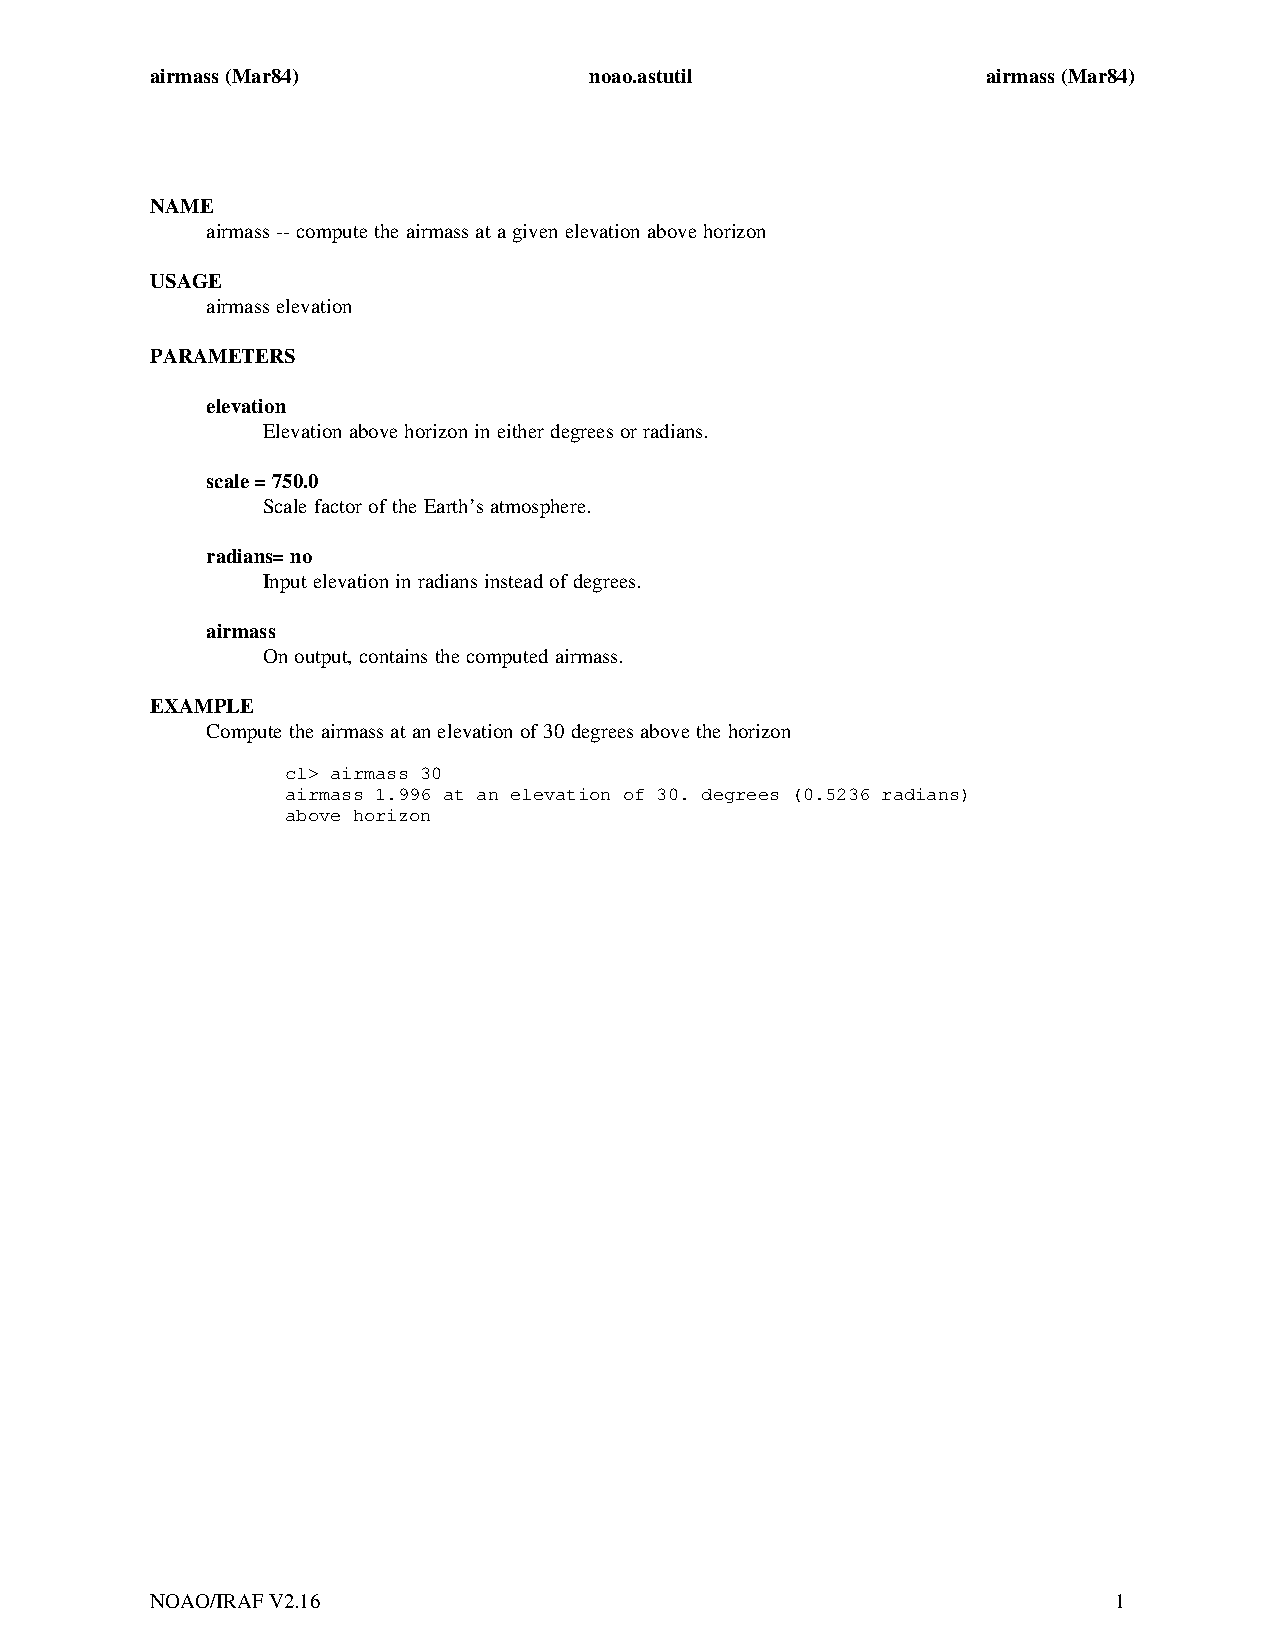
\includepdf[pages=-,addtotoc={1,section,1,airmass,sec:airmass}]{airmass.pdf}

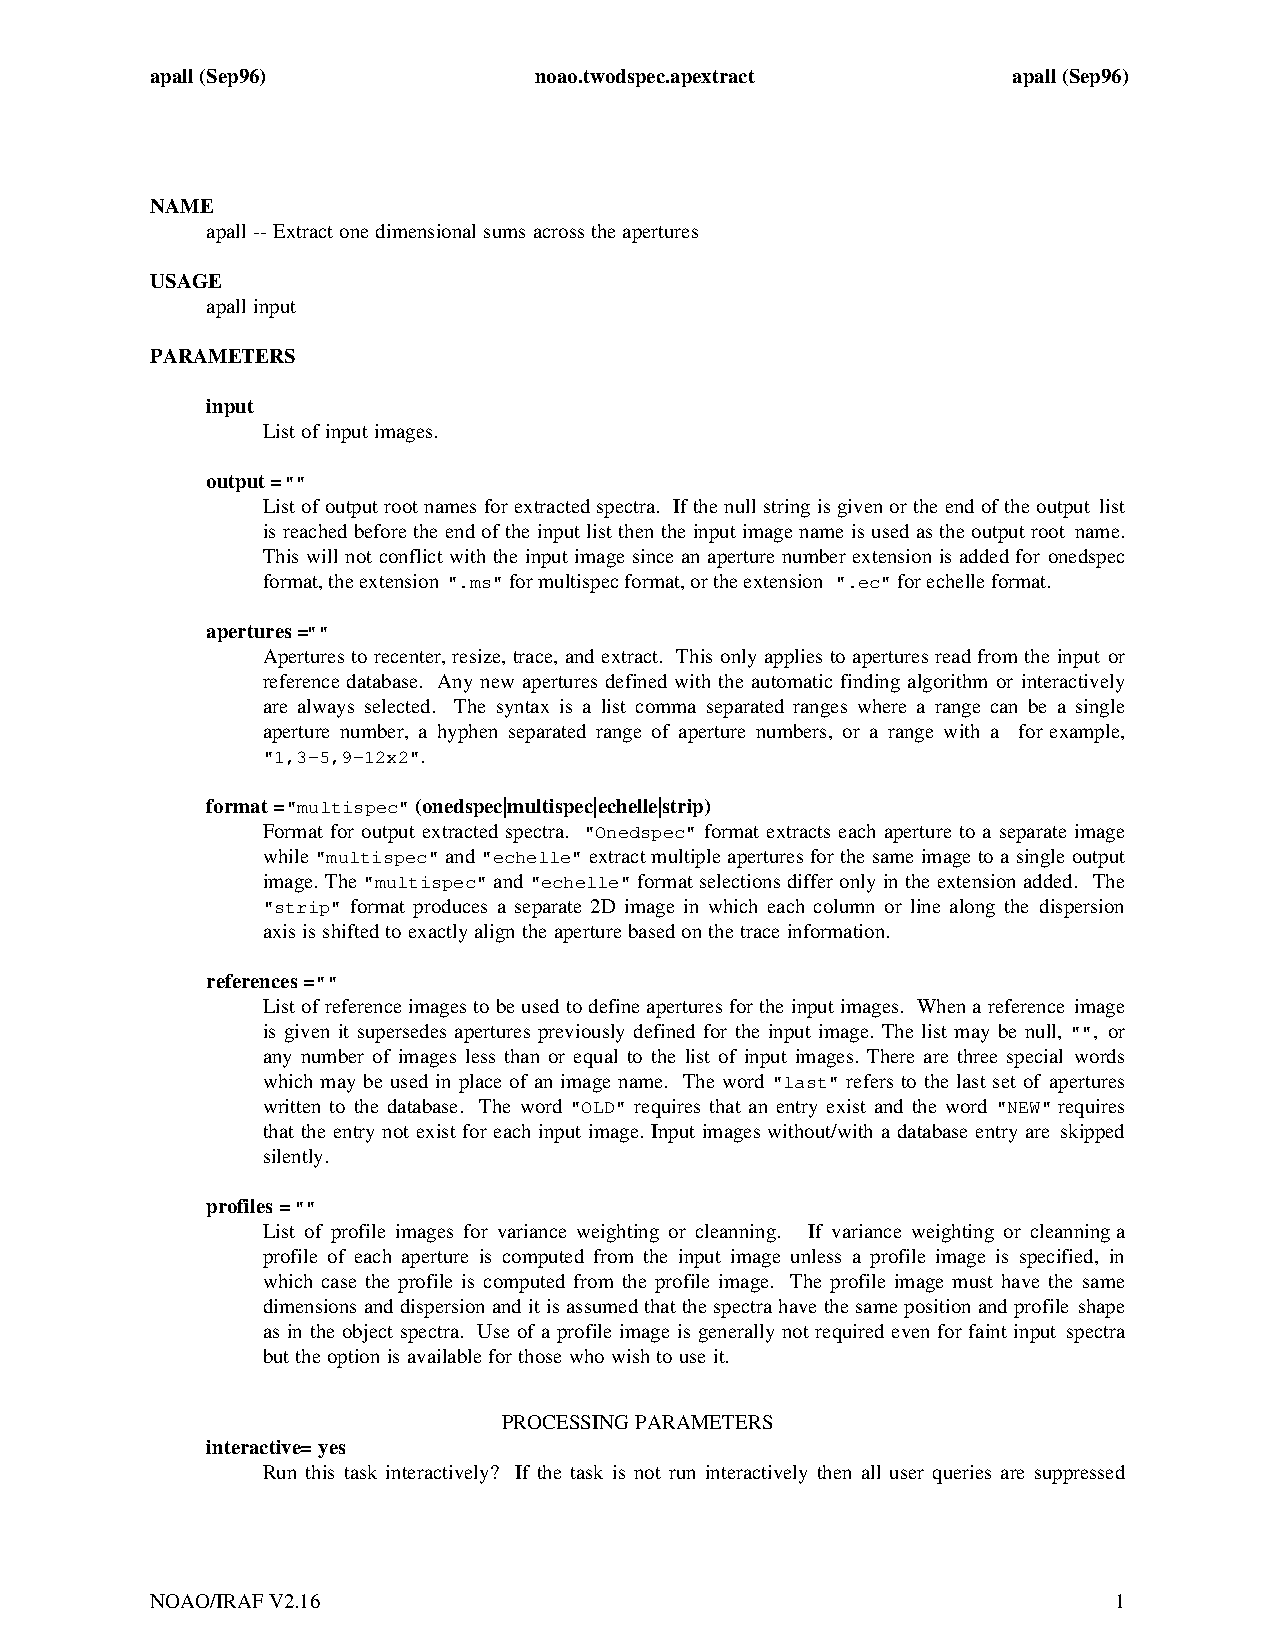
\includepdf[pages=-,addtotoc={1,section,1,apall,sec:apall}]{apall.pdf}

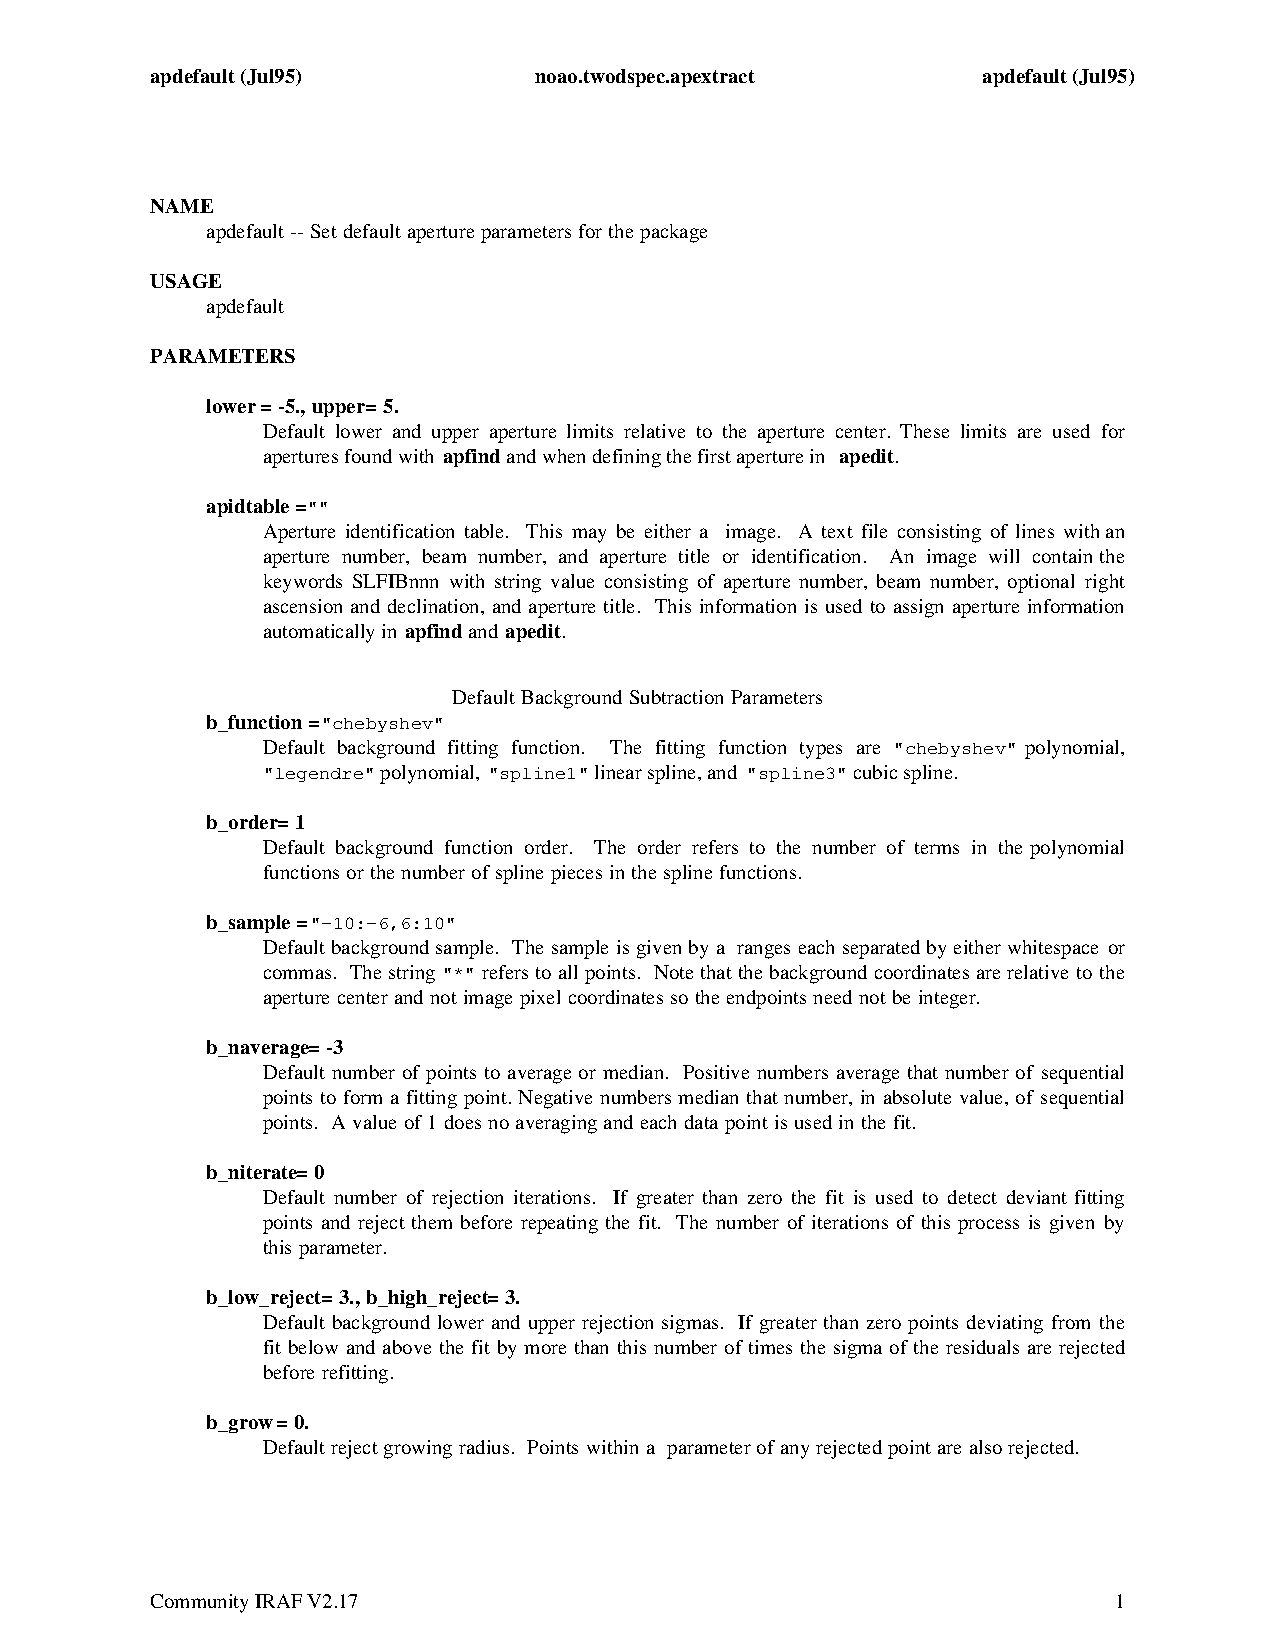
\includepdf[pages=-,addtotoc={1,section,1,apdefault,sec:apdefault}]{apdefault.pdf}

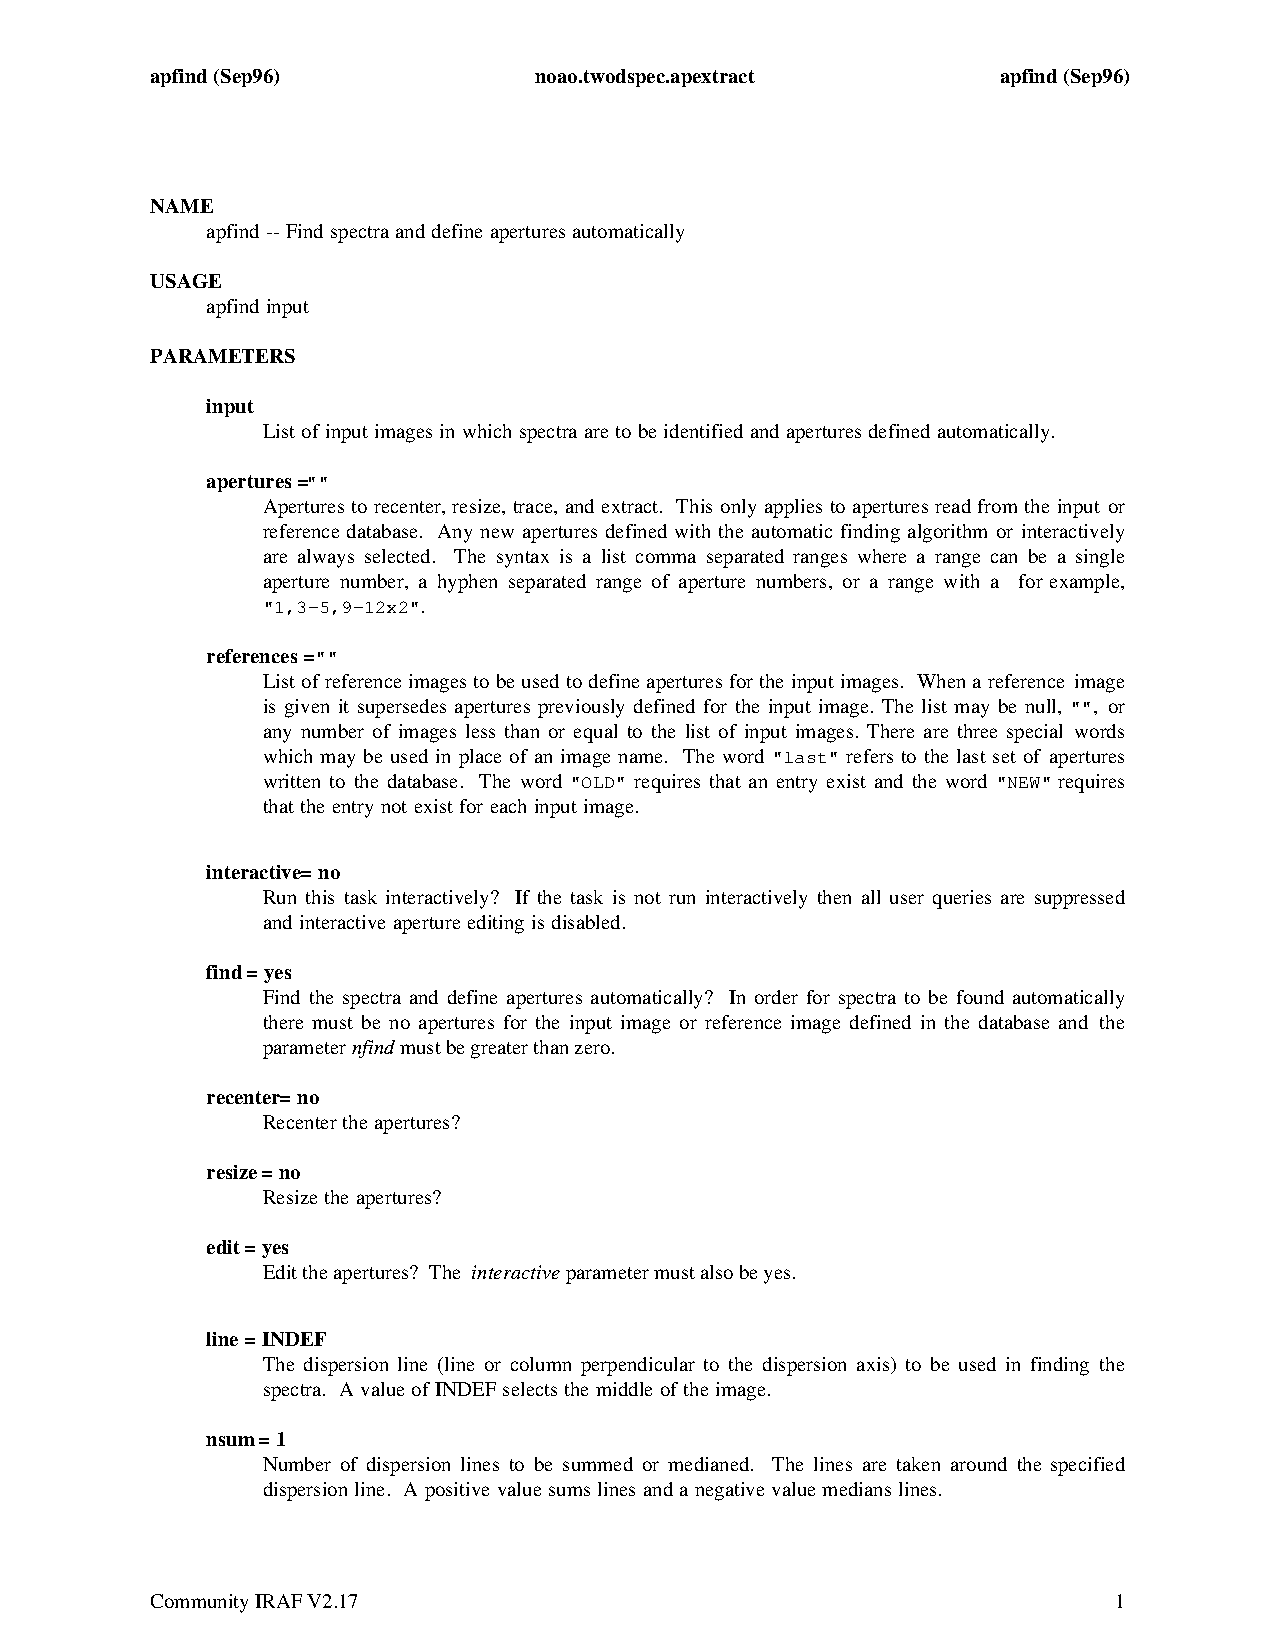
\includepdf[pages=-,addtotoc={1,section,1,apfind,sec:apfind}]{apfind.pdf}

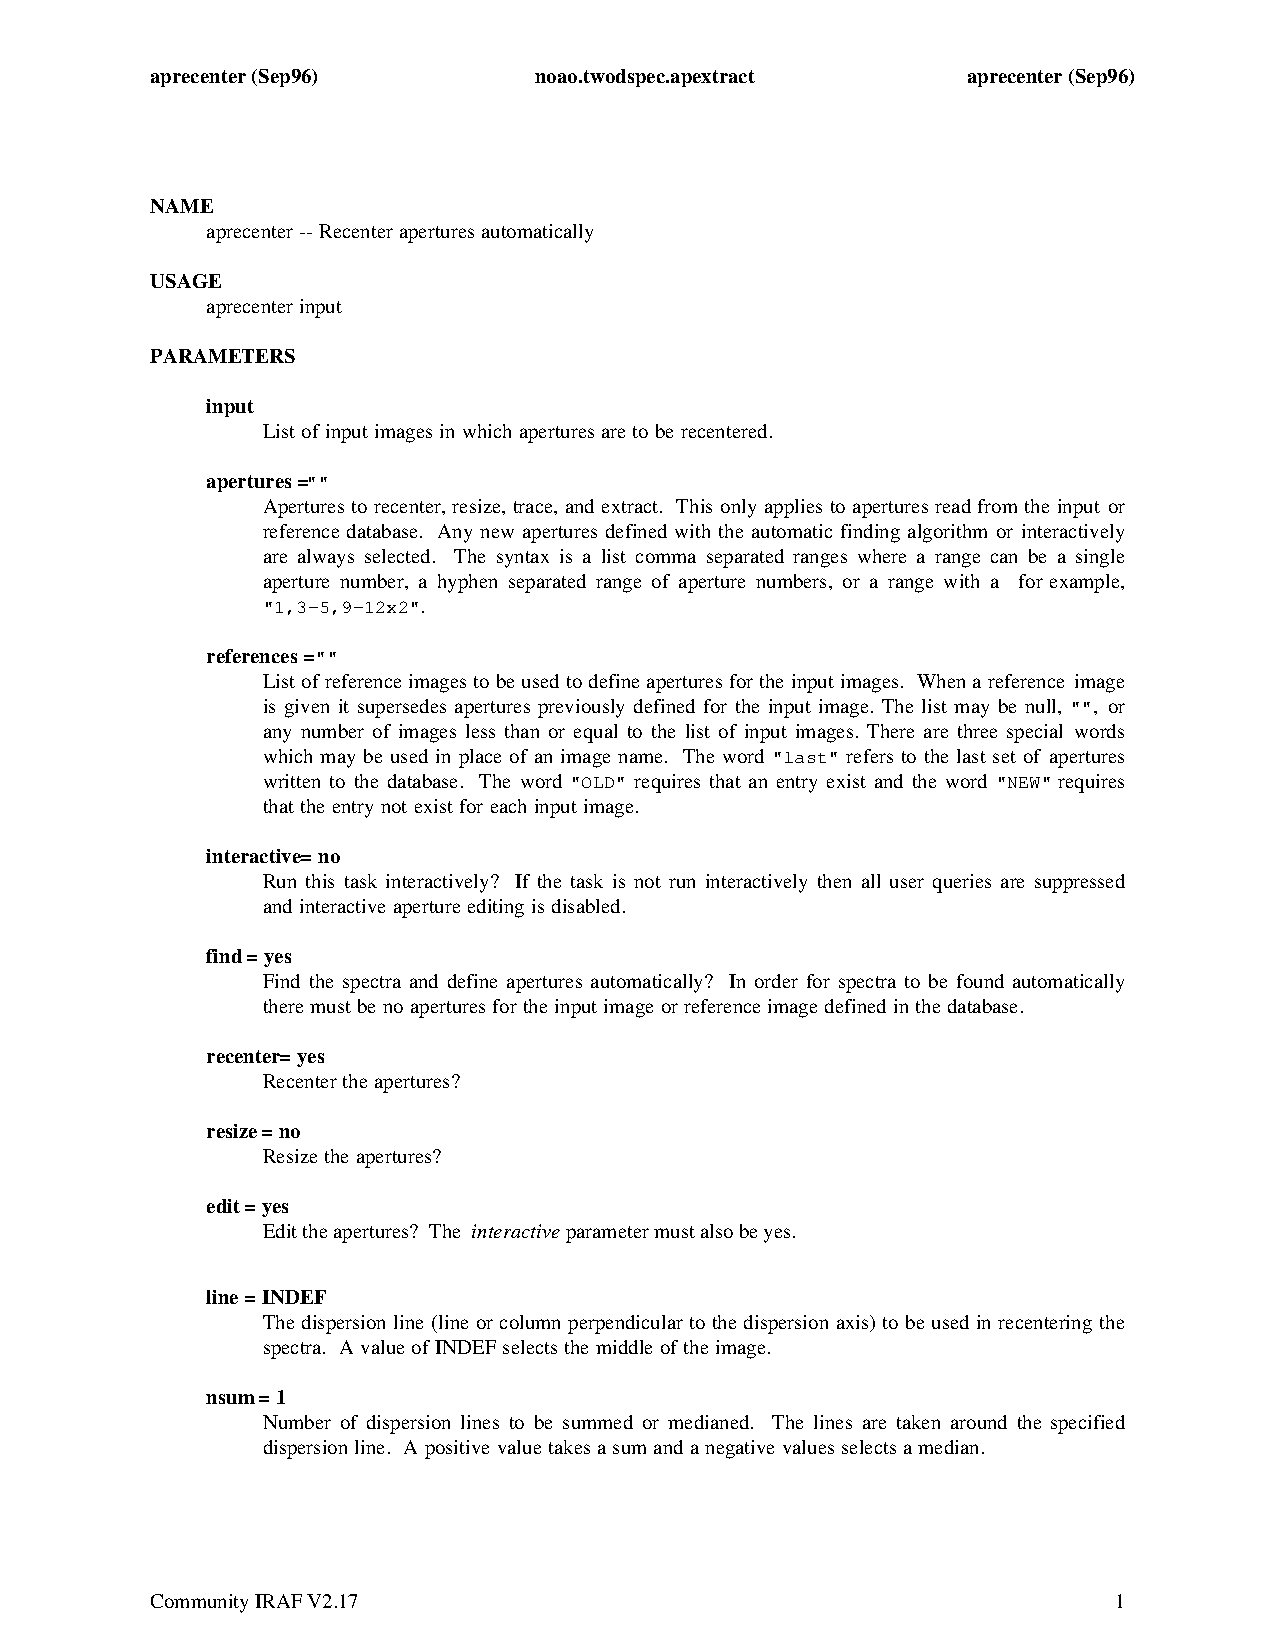
\includepdf[pages=-,addtotoc={1,section,1,aprecenter,sec:aprecenter}]{aprecenter.pdf}

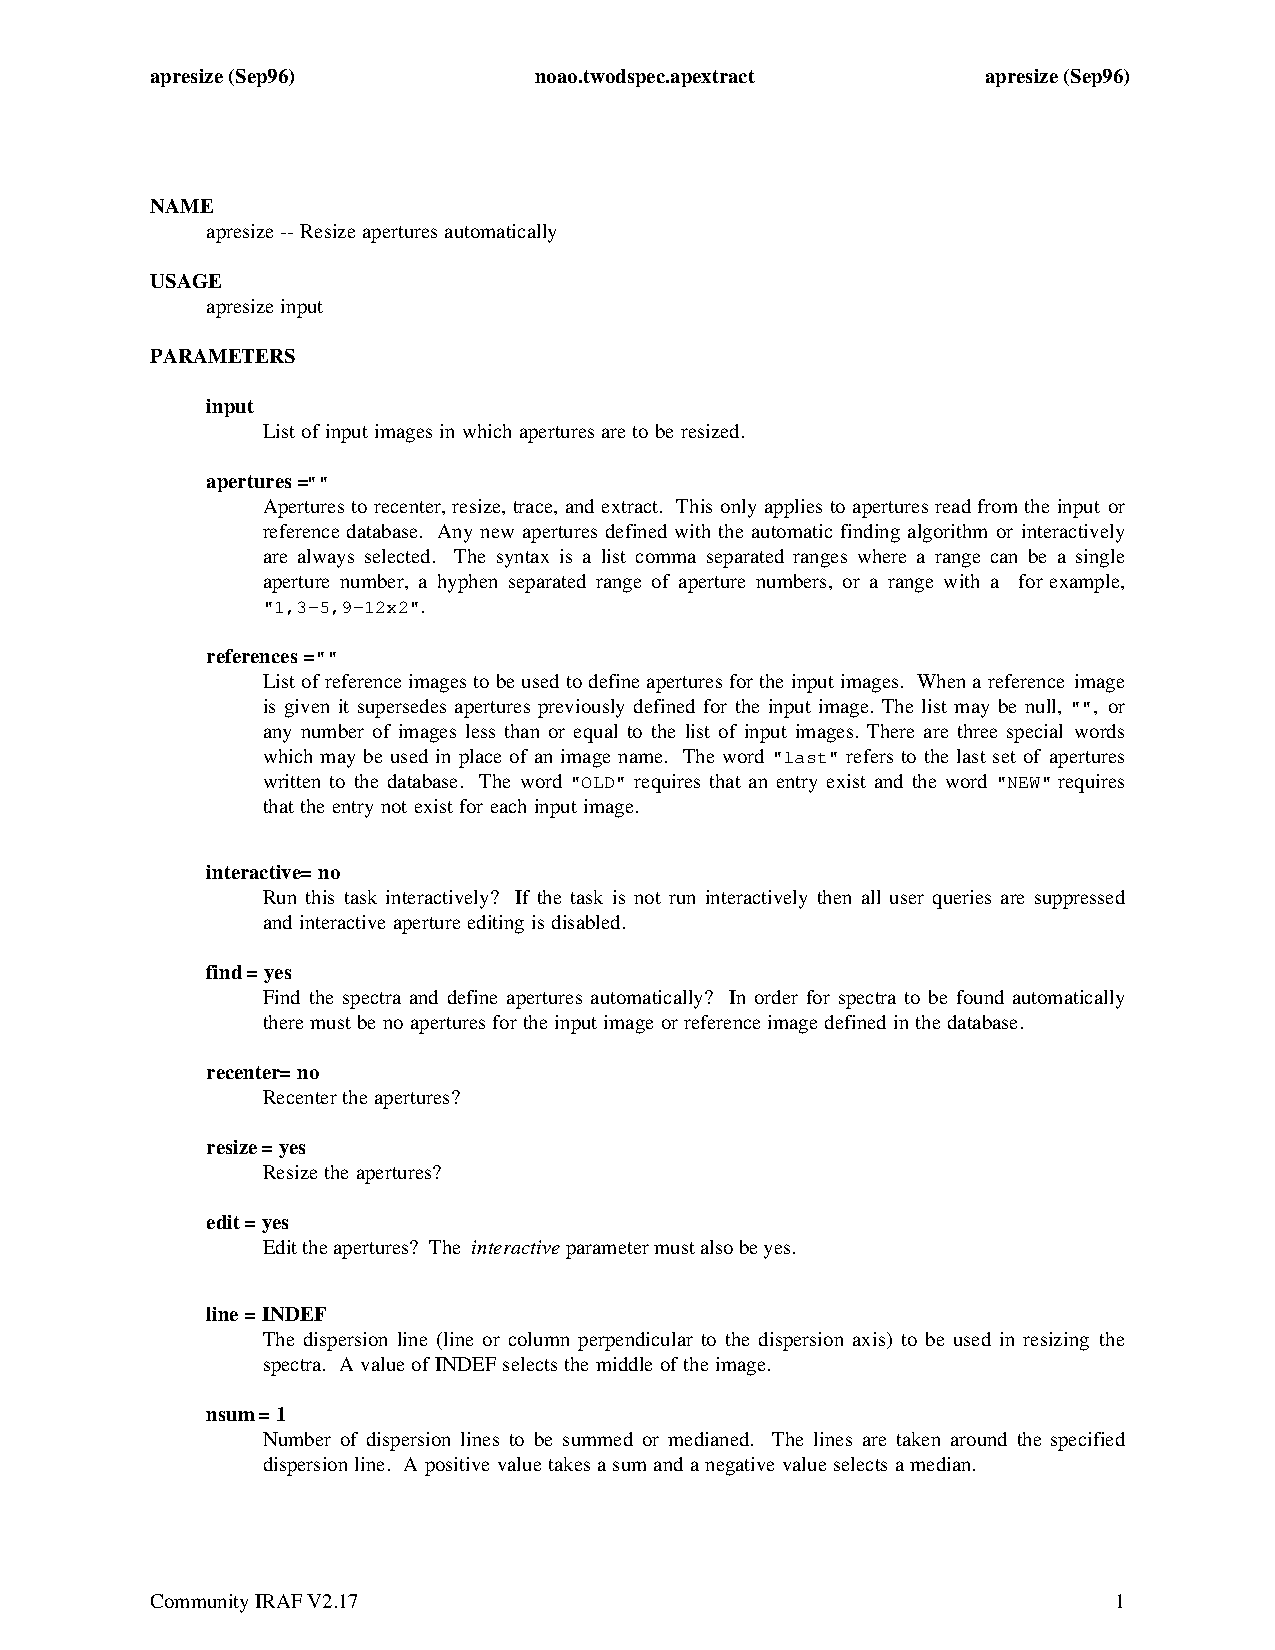
\includepdf[pages=-,addtotoc={1,section,1,apresize,sec:apresize}]{apresize.pdf}

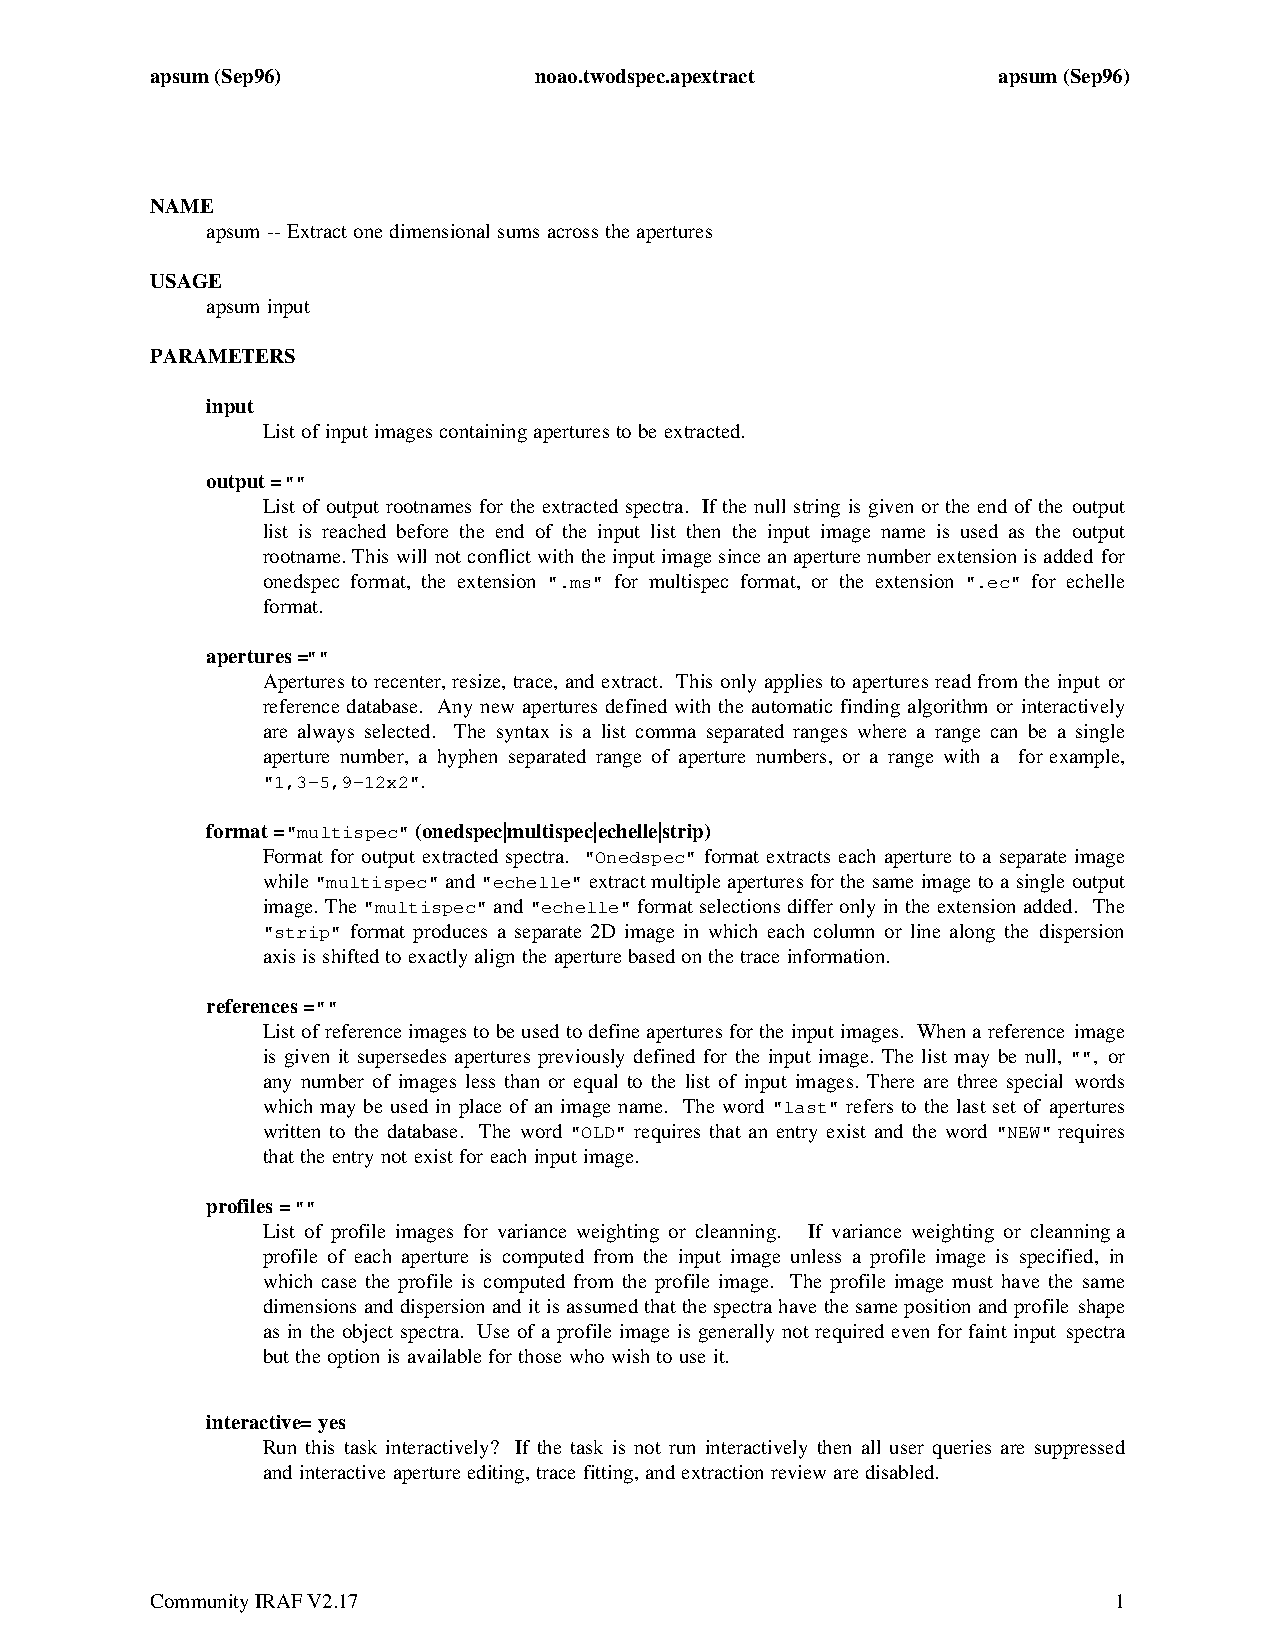
\includepdf[pages=-,addtotoc={1,section,1,apsum,sec:apsum}]{apsum.pdf}

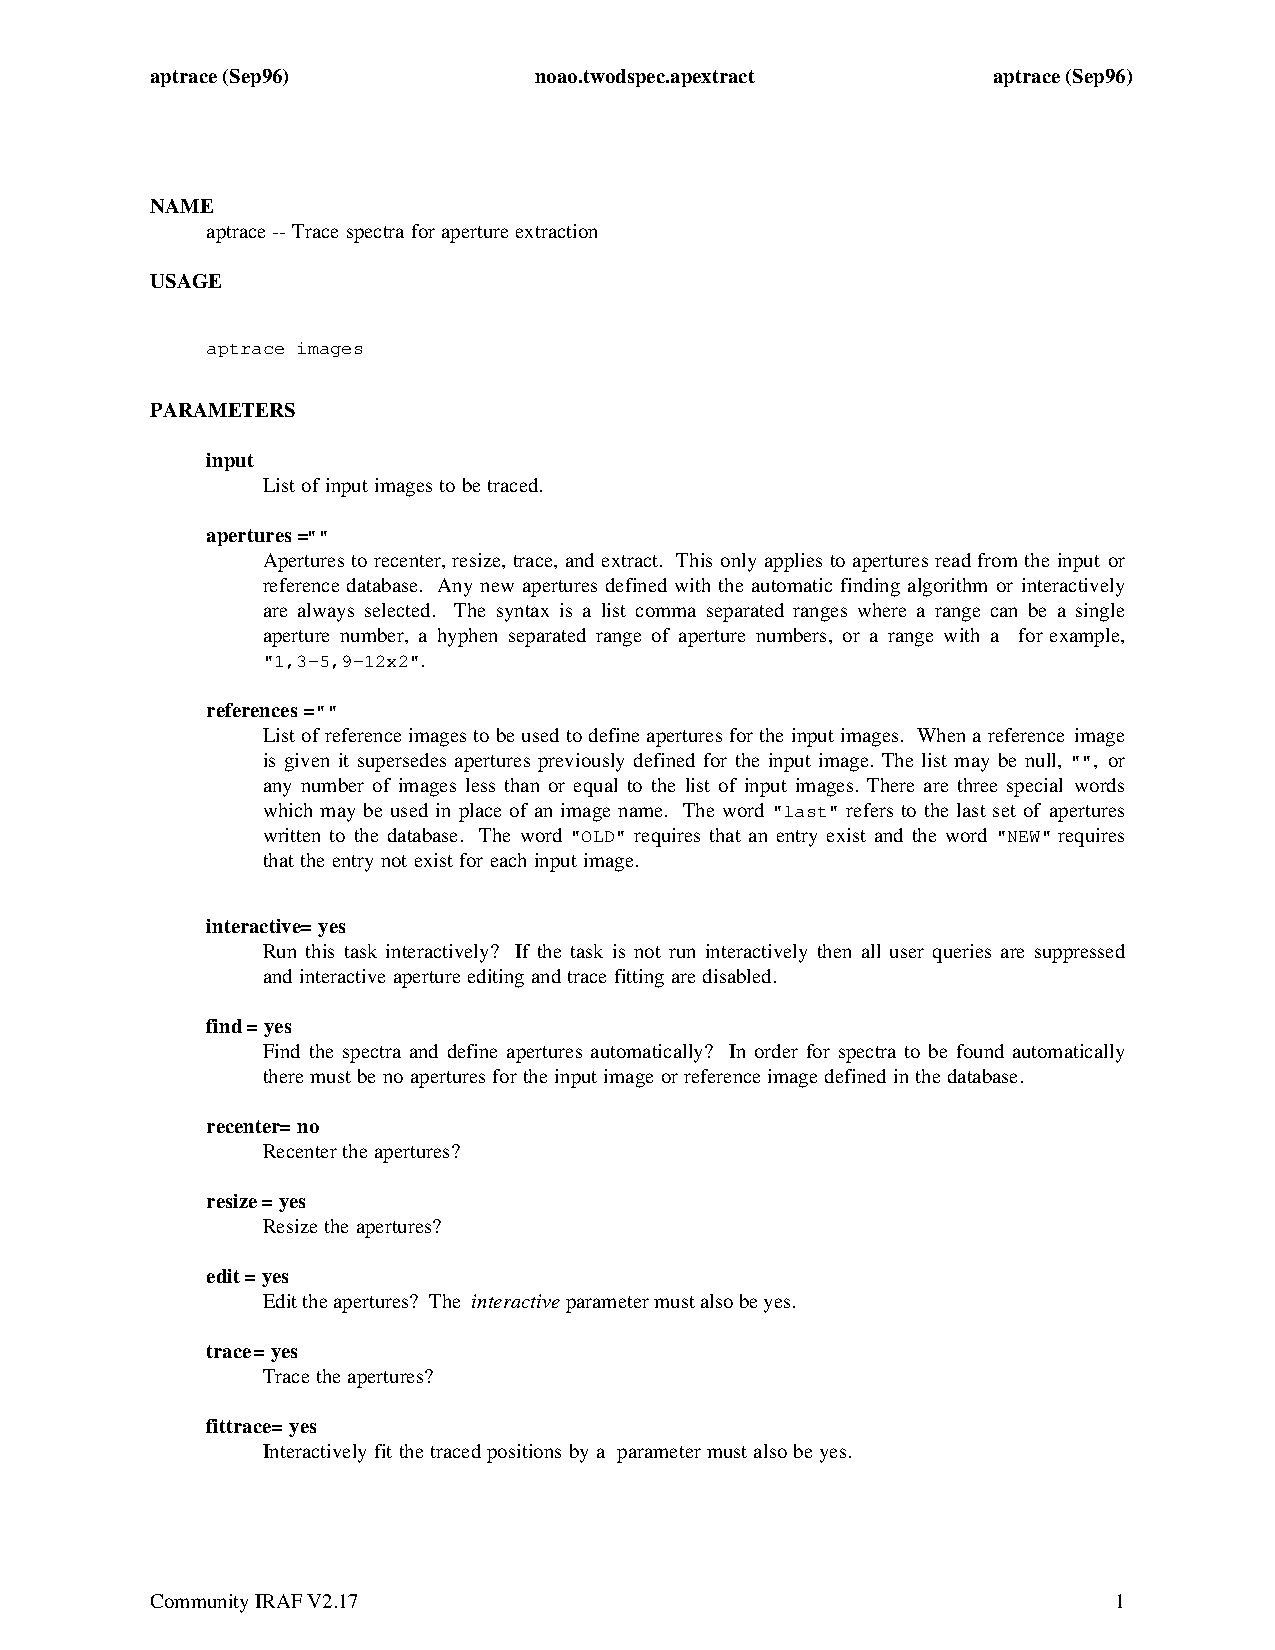
\includepdf[pages=-,addtotoc={1,section,1,aptrace,sec:aptrace}]{aptrace.pdf}

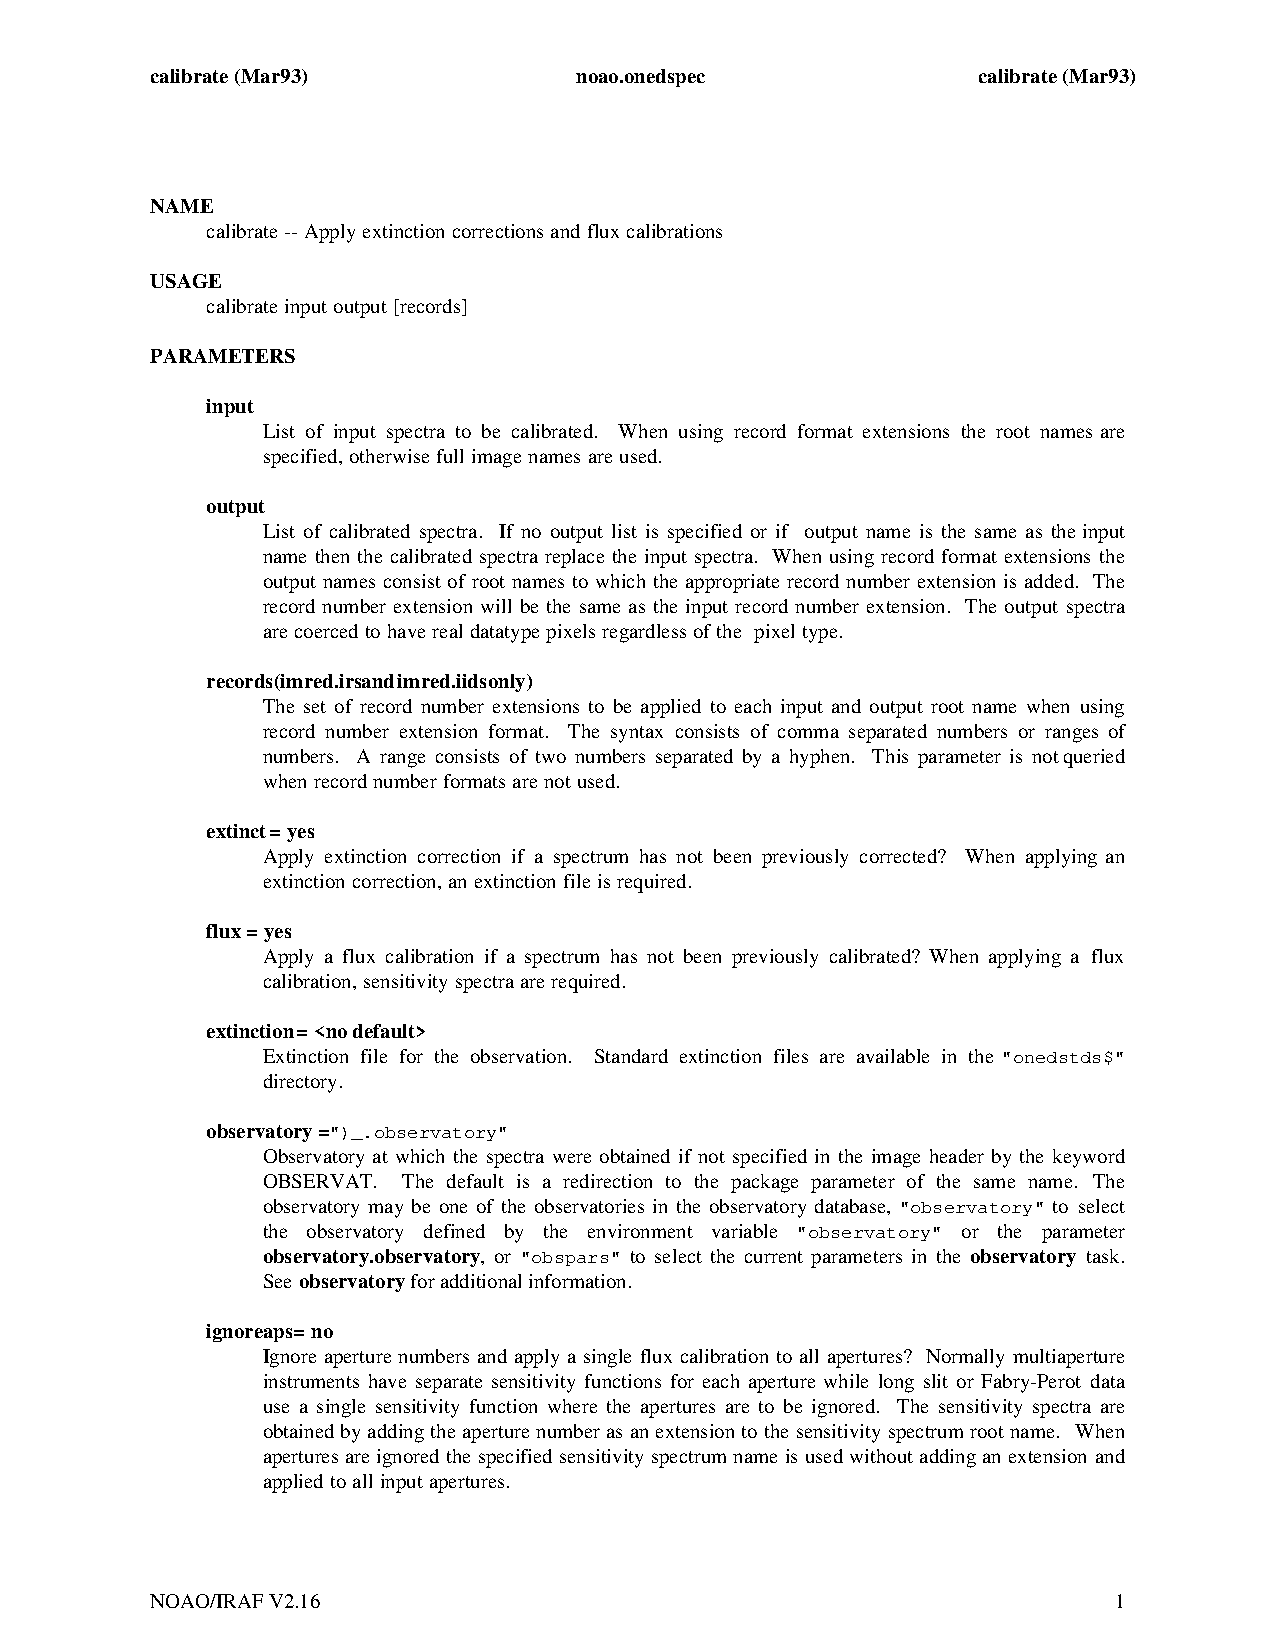
\includepdf[pages=-,addtotoc={1,section,1,calibrate,sec:calibrate}]{calibrate.pdf}

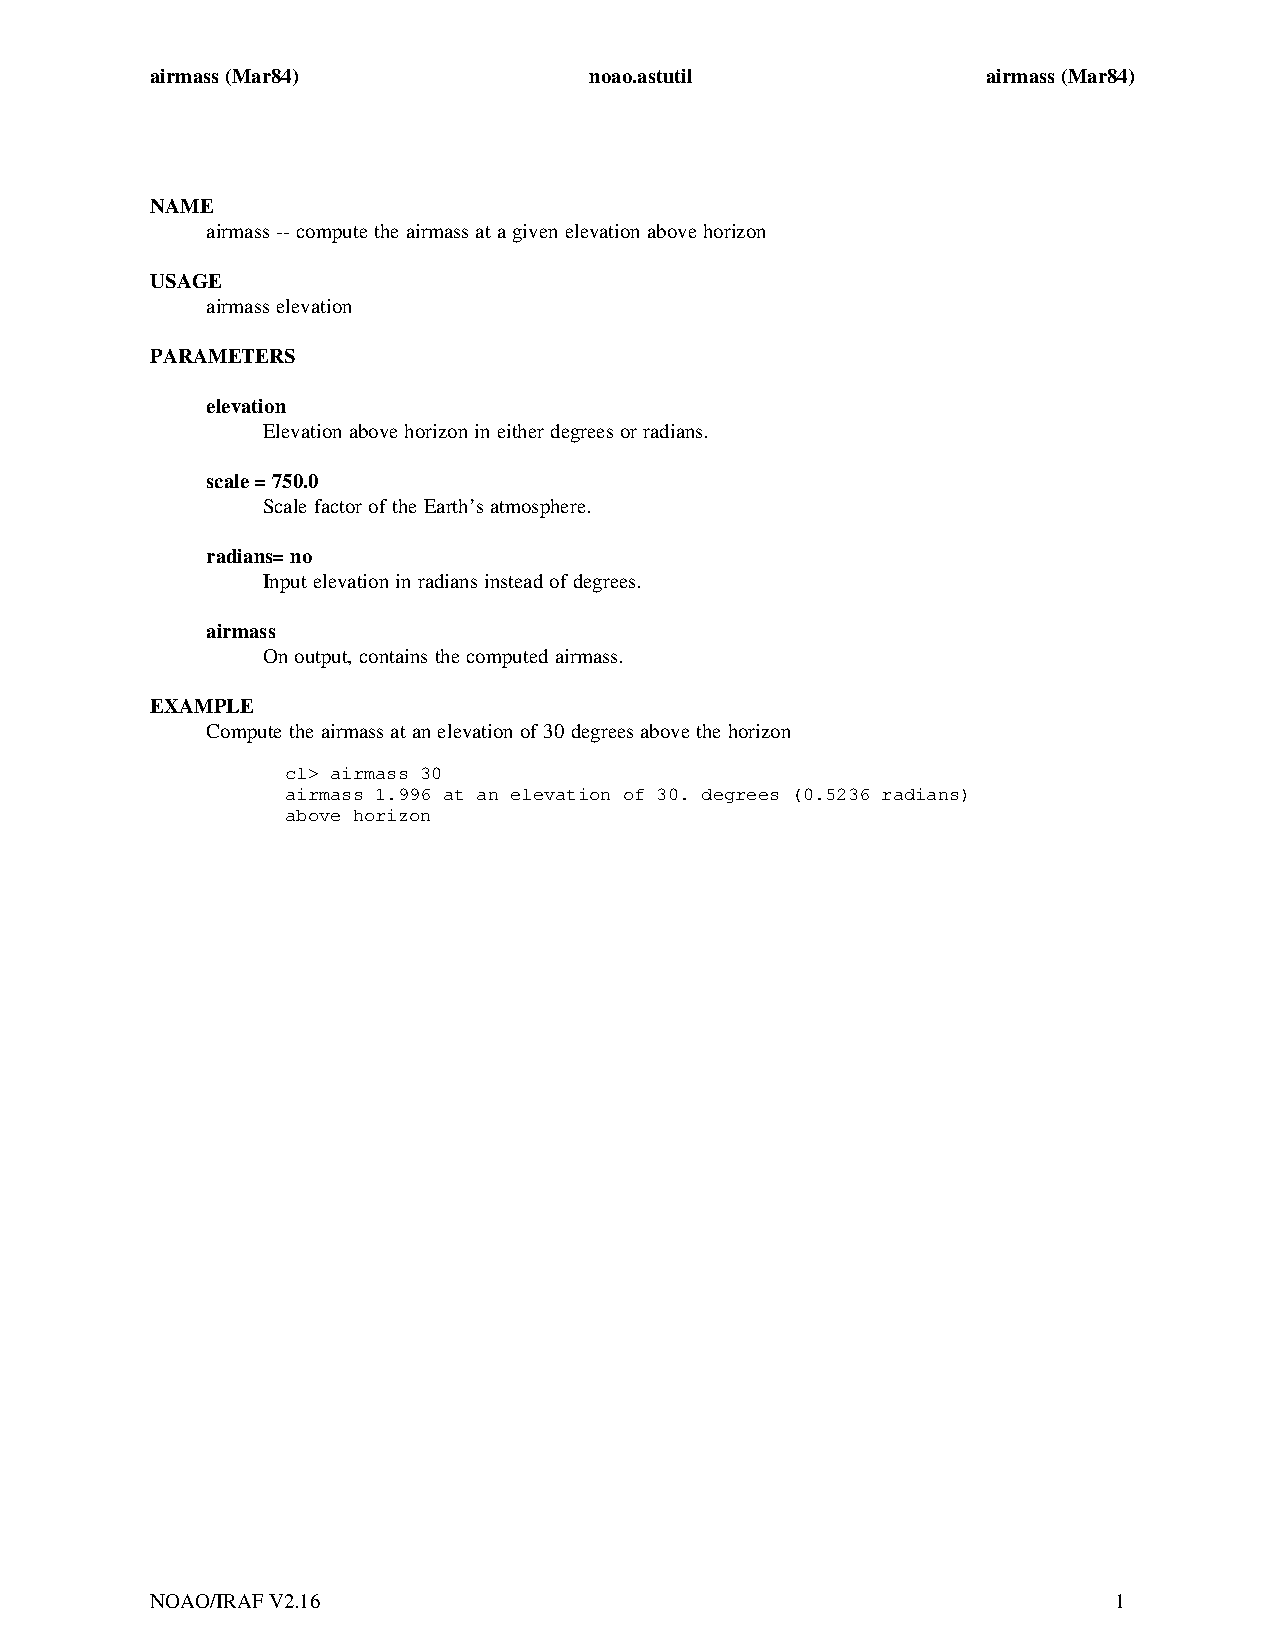
\includepdf[pages=-,addtotoc={1,section,1,combined,sec:combined}]{combined.pdf}

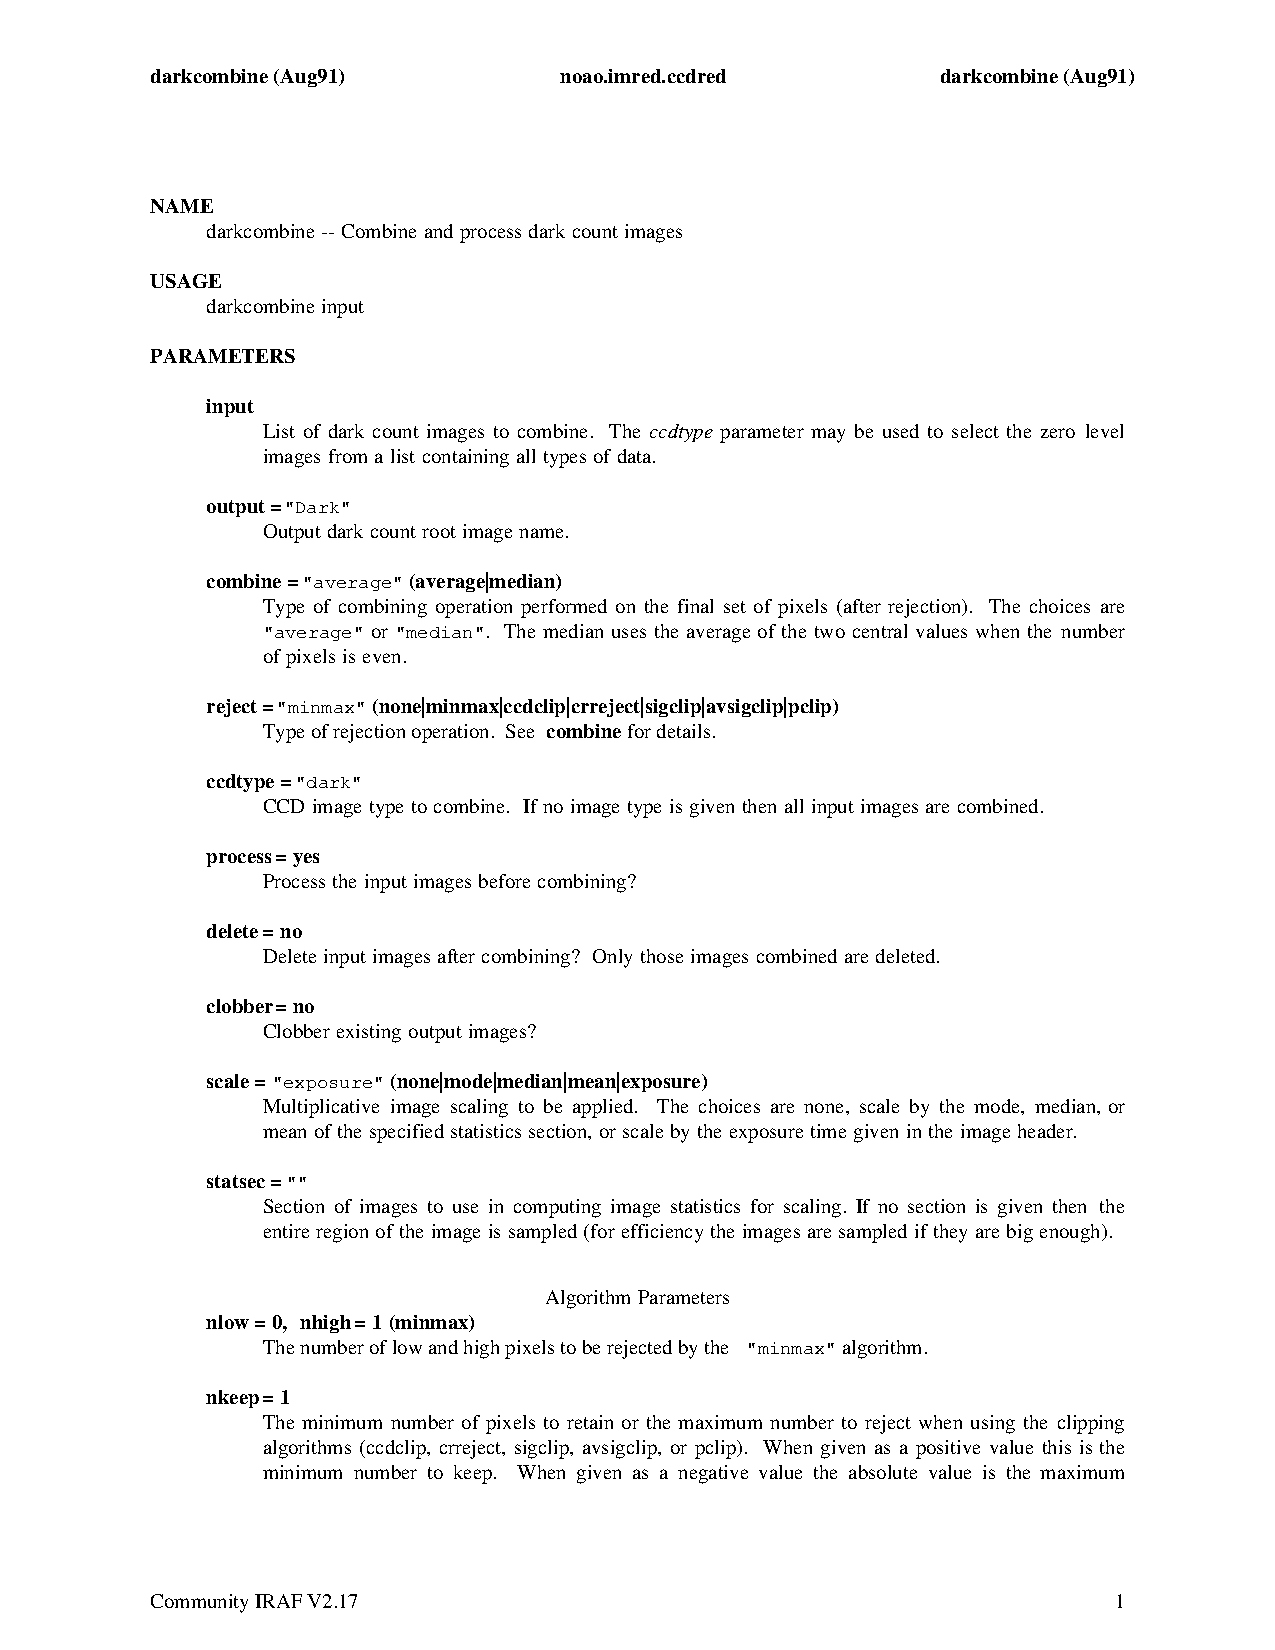
\includepdf[pages=-,addtotoc={1,section,1,darkcombine,sec:darkcombine}]{darkcombine.pdf}

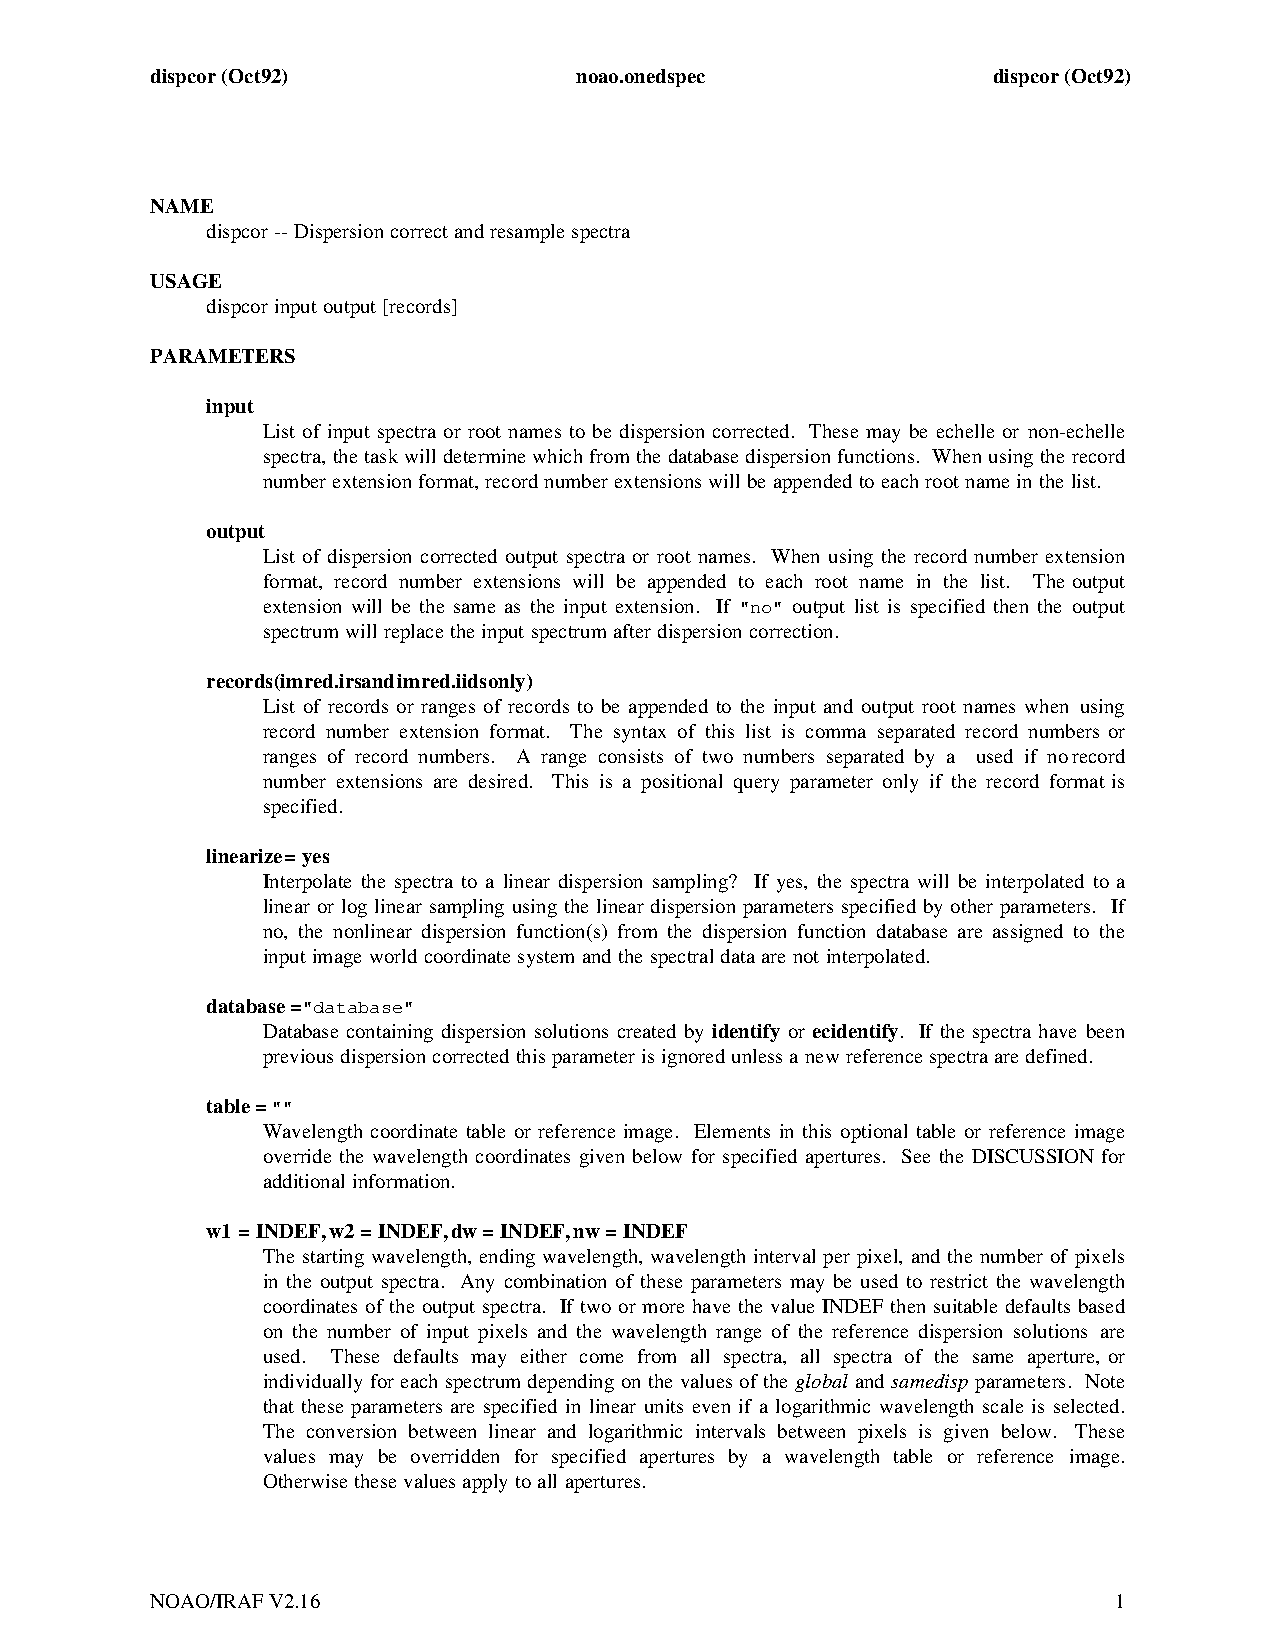
\includepdf[pages=-,addtotoc={1,section,1,dispcor,sec:dispcor}]{dispcor.pdf}

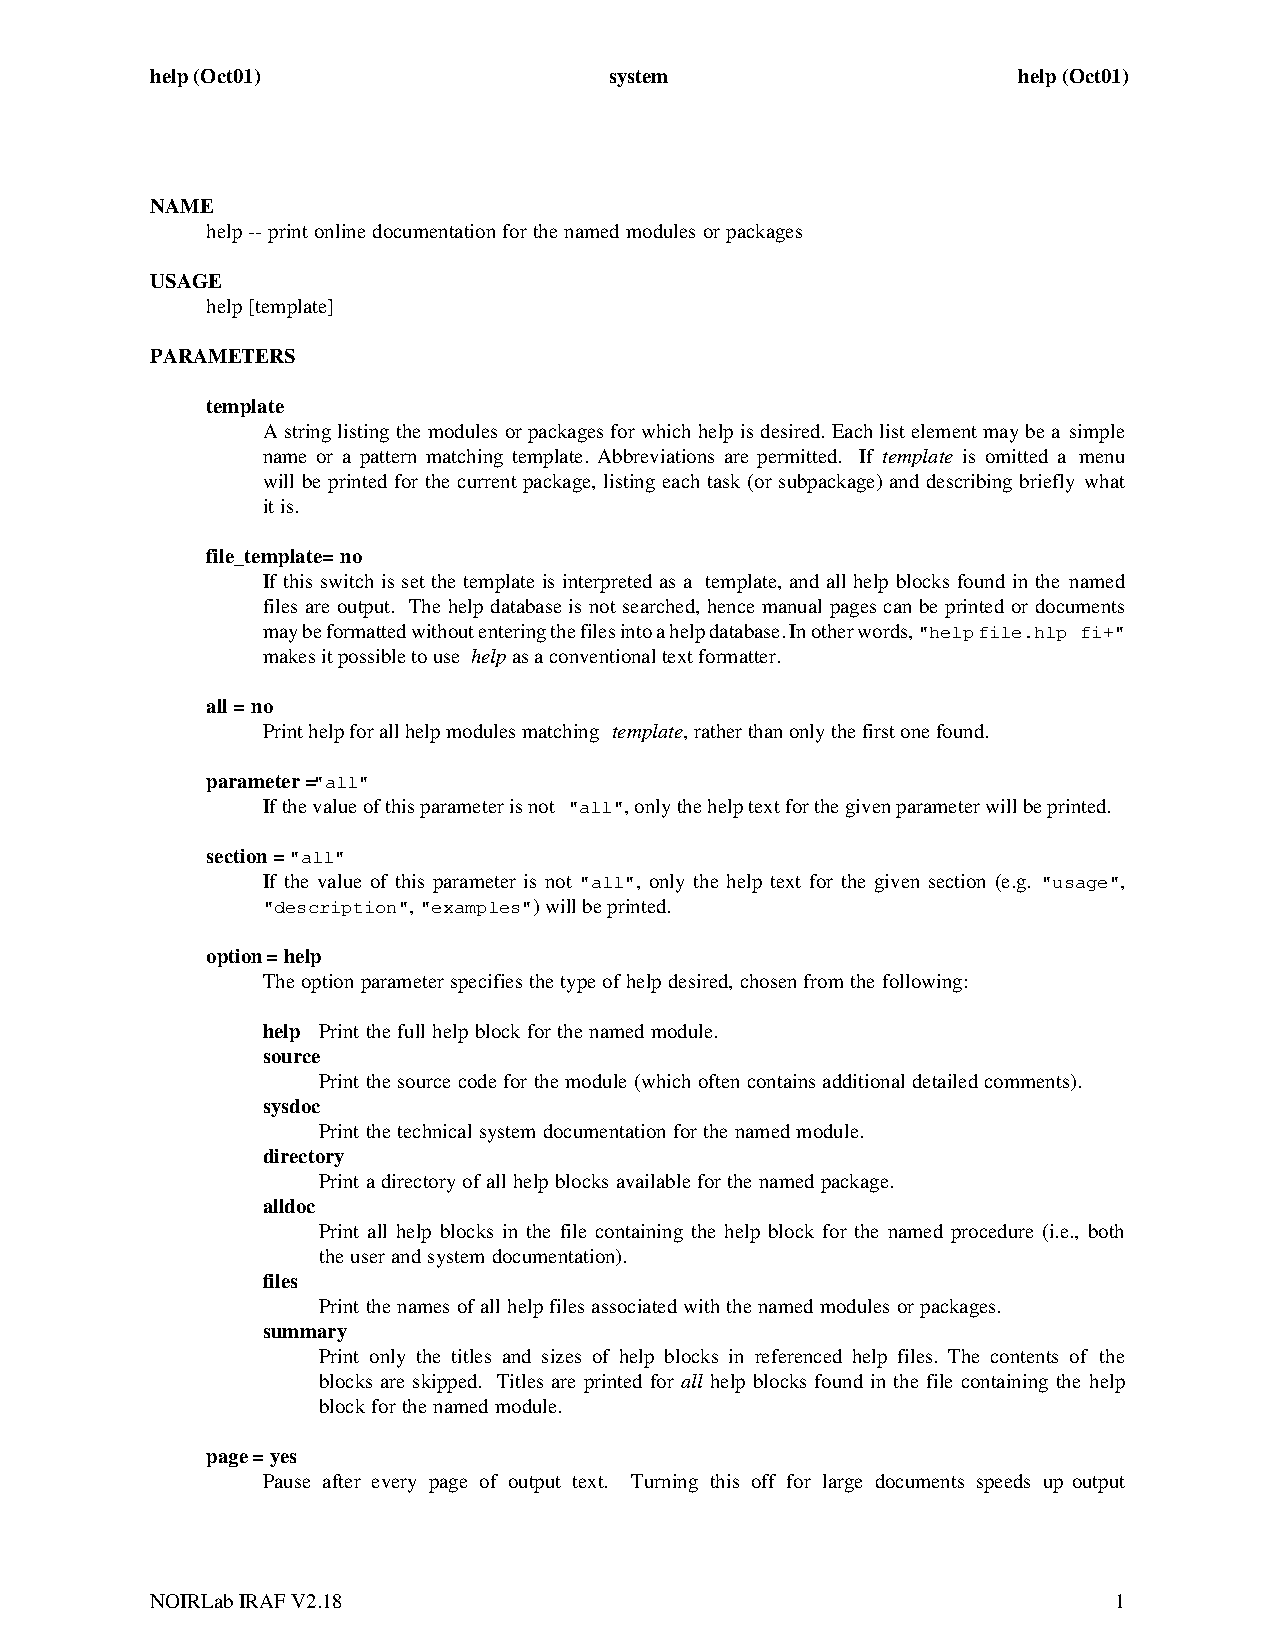
\includepdf[pages=-,addtotoc={1,section,1,help,sec:help}]{help.pdf}


\includepdf[pages=-,addtotoc={1,section,1,identify,sec:identify}]{identify.pdf}

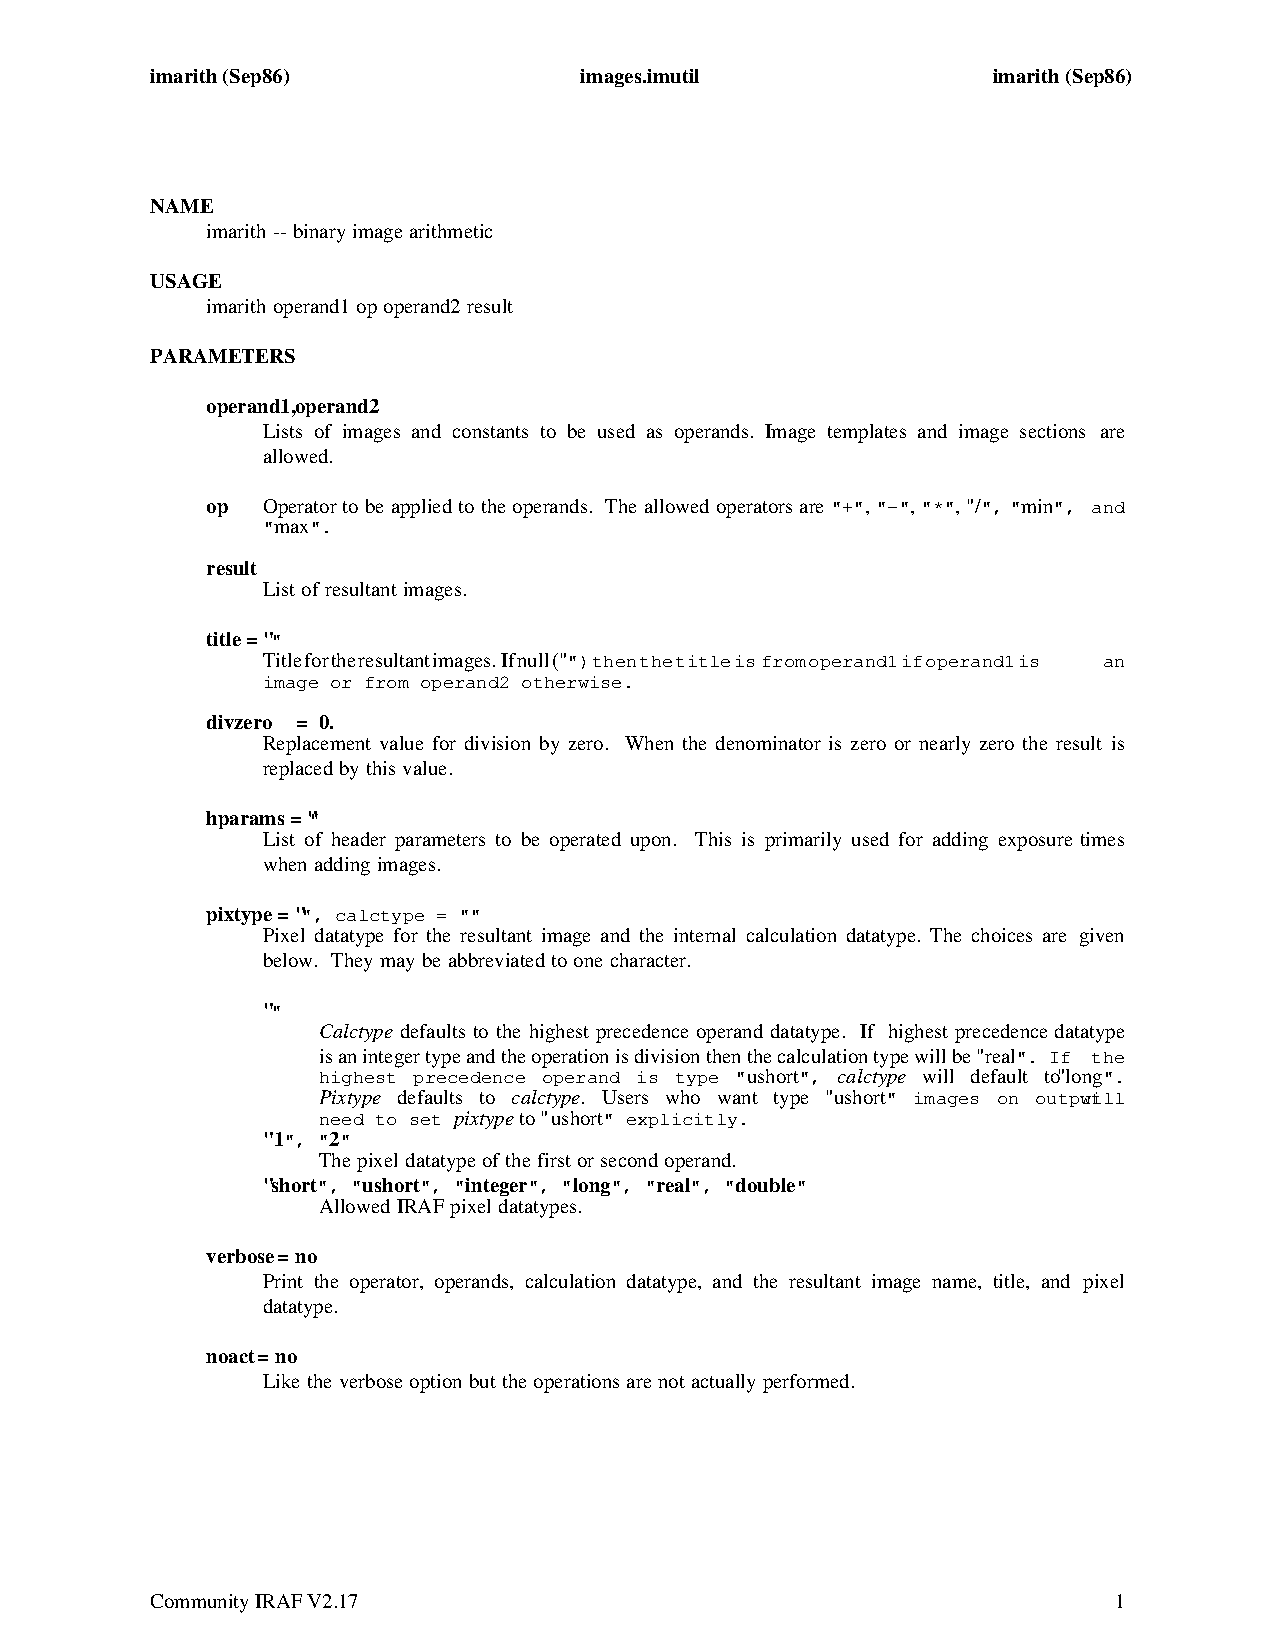
\includepdf[pages=-,addtotoc={1,section,1,imarith,sec:imarith}]{imarith.pdf}

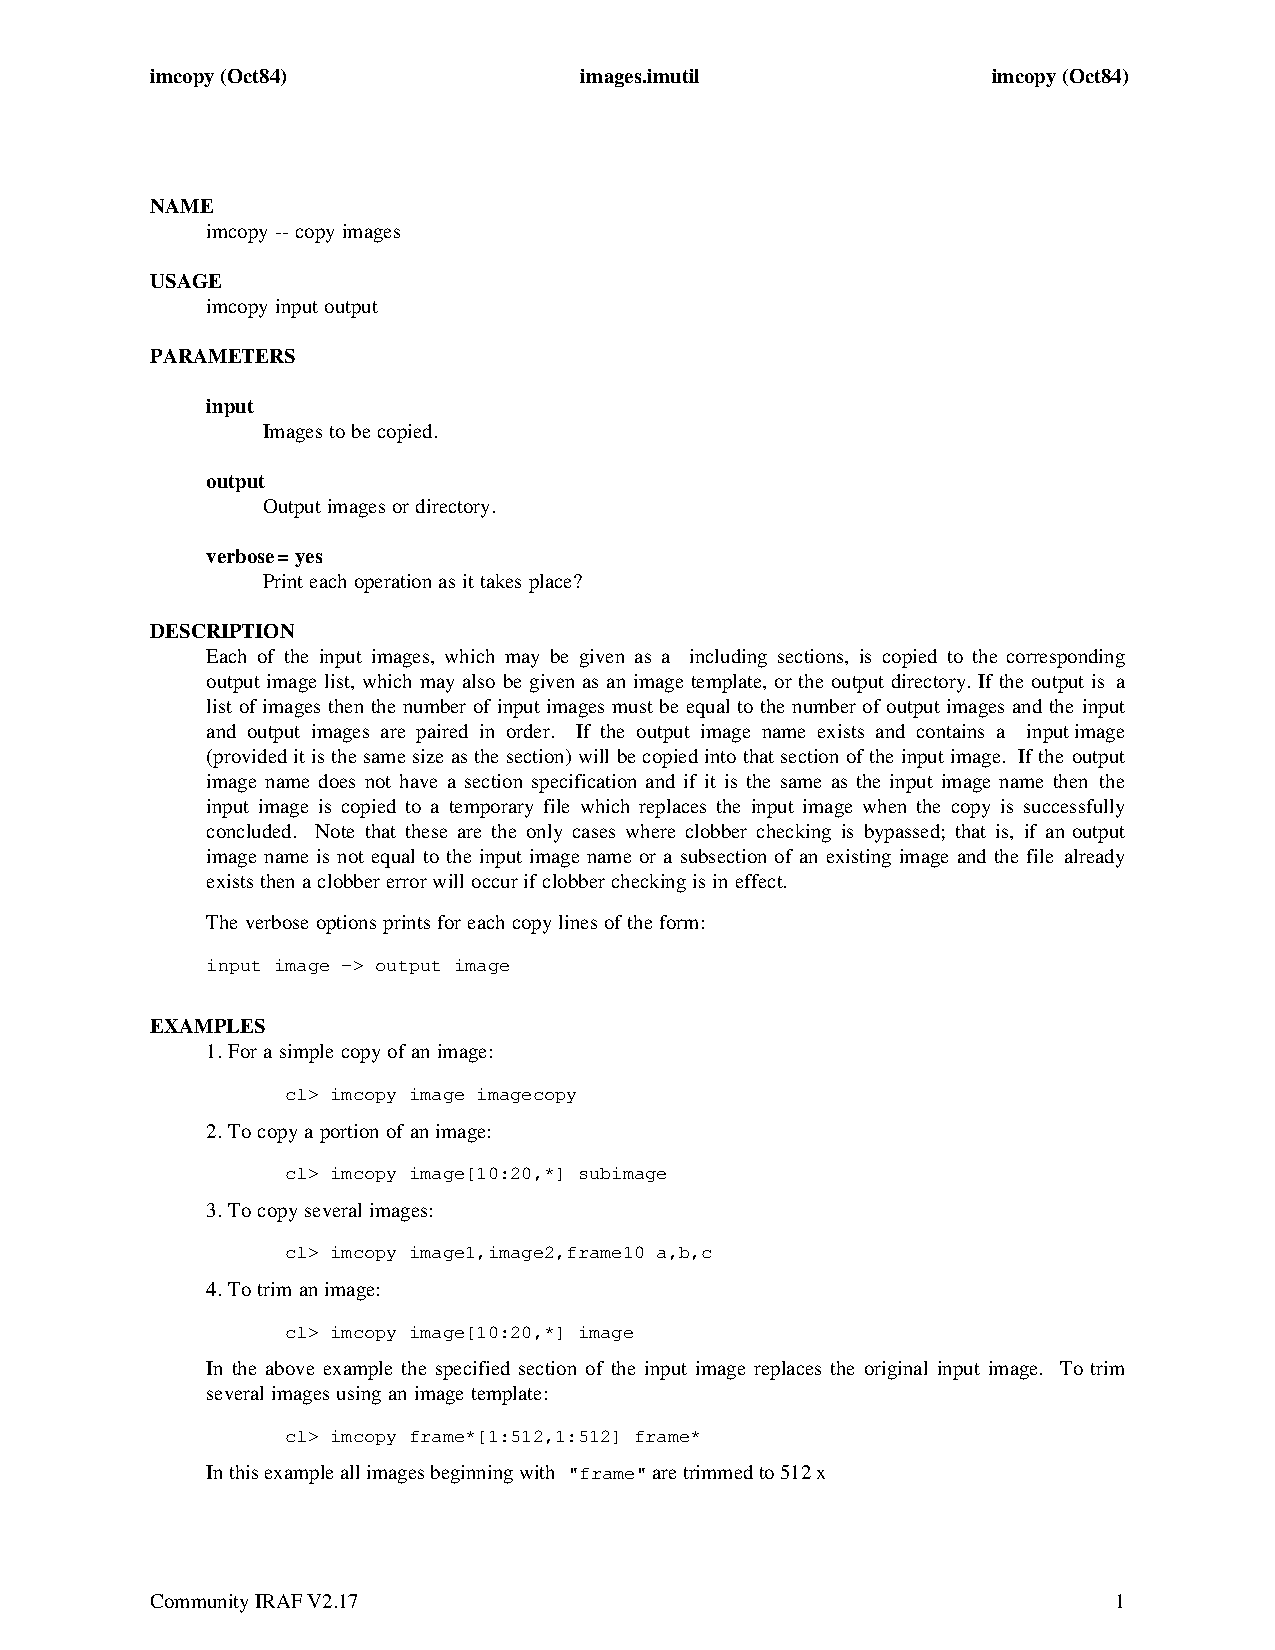
\includepdf[pages=-,addtotoc={1,section,1,imcopy,sec:imcopy}]{imcopy.pdf}

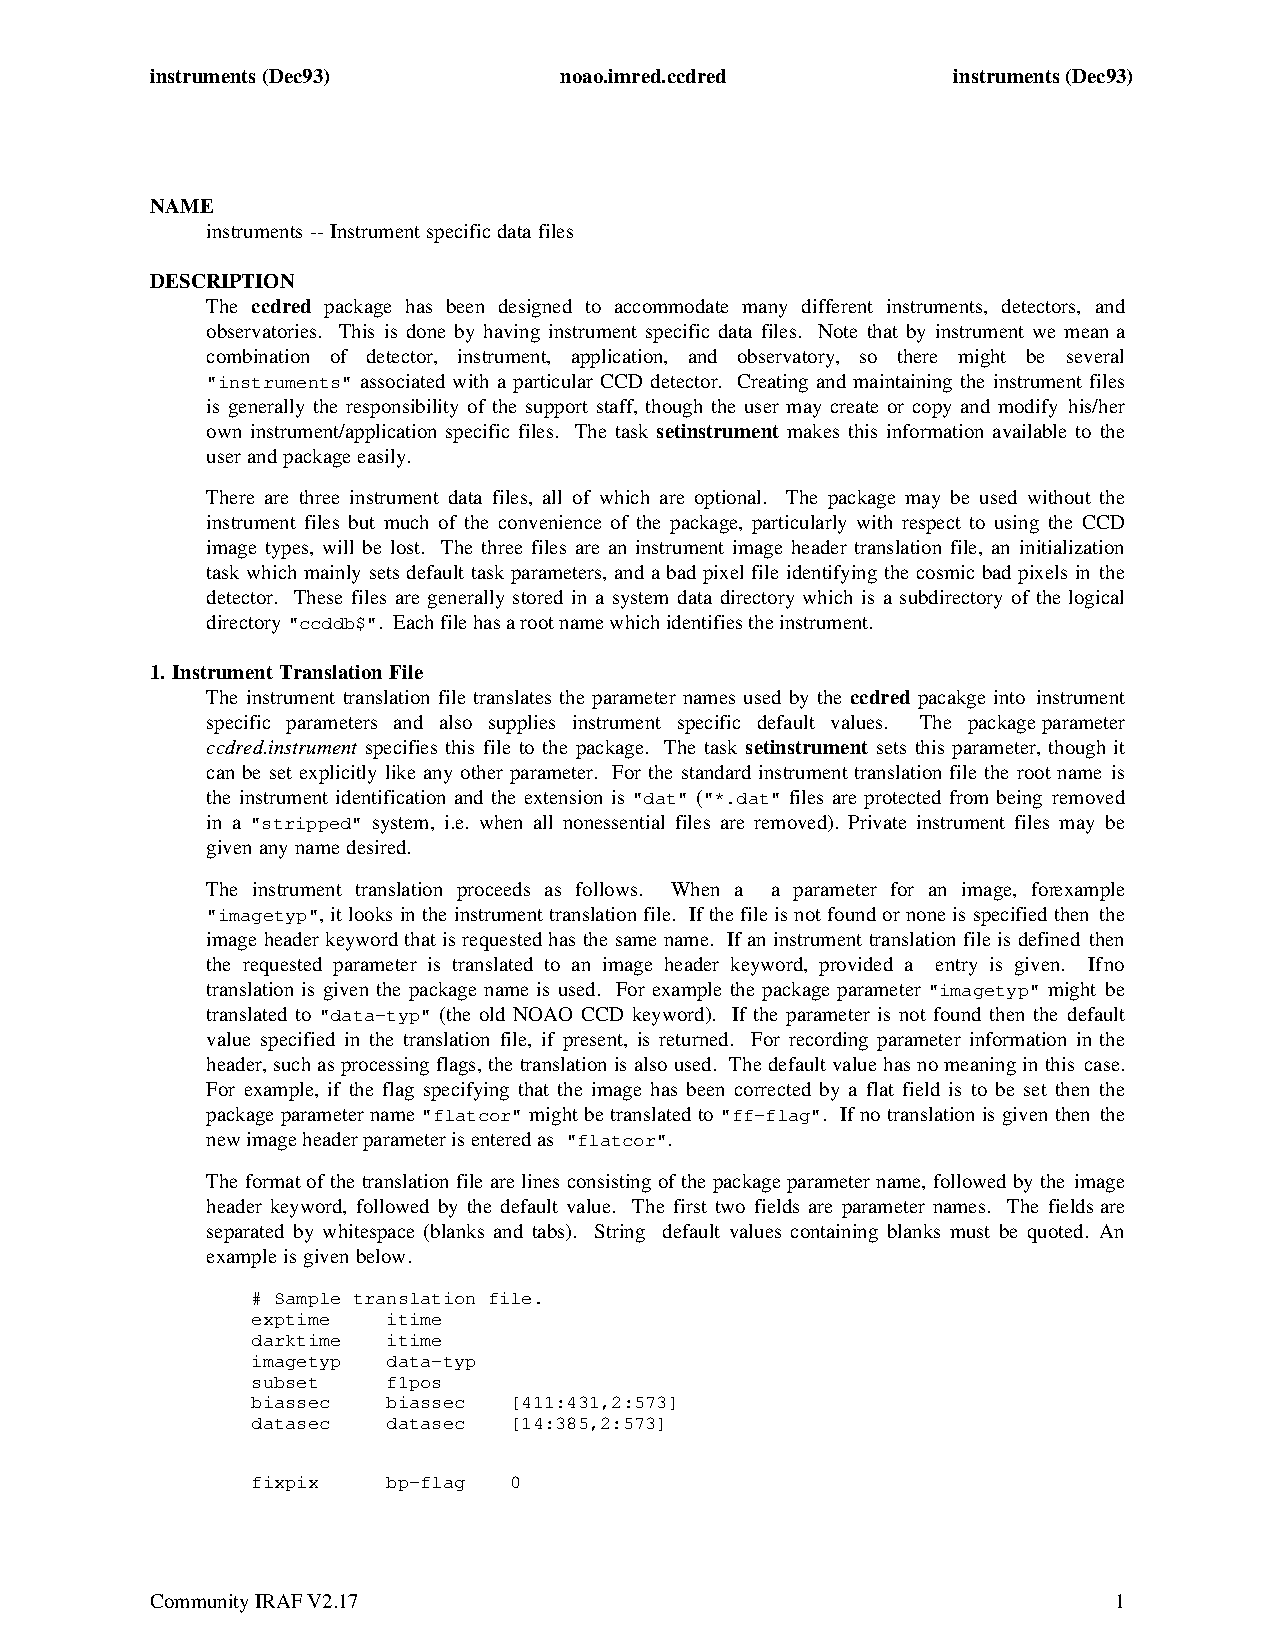
\includepdf[pages=-,addtotoc={1,section,1,instruments,sec:instruments}]{instruments.pdf}

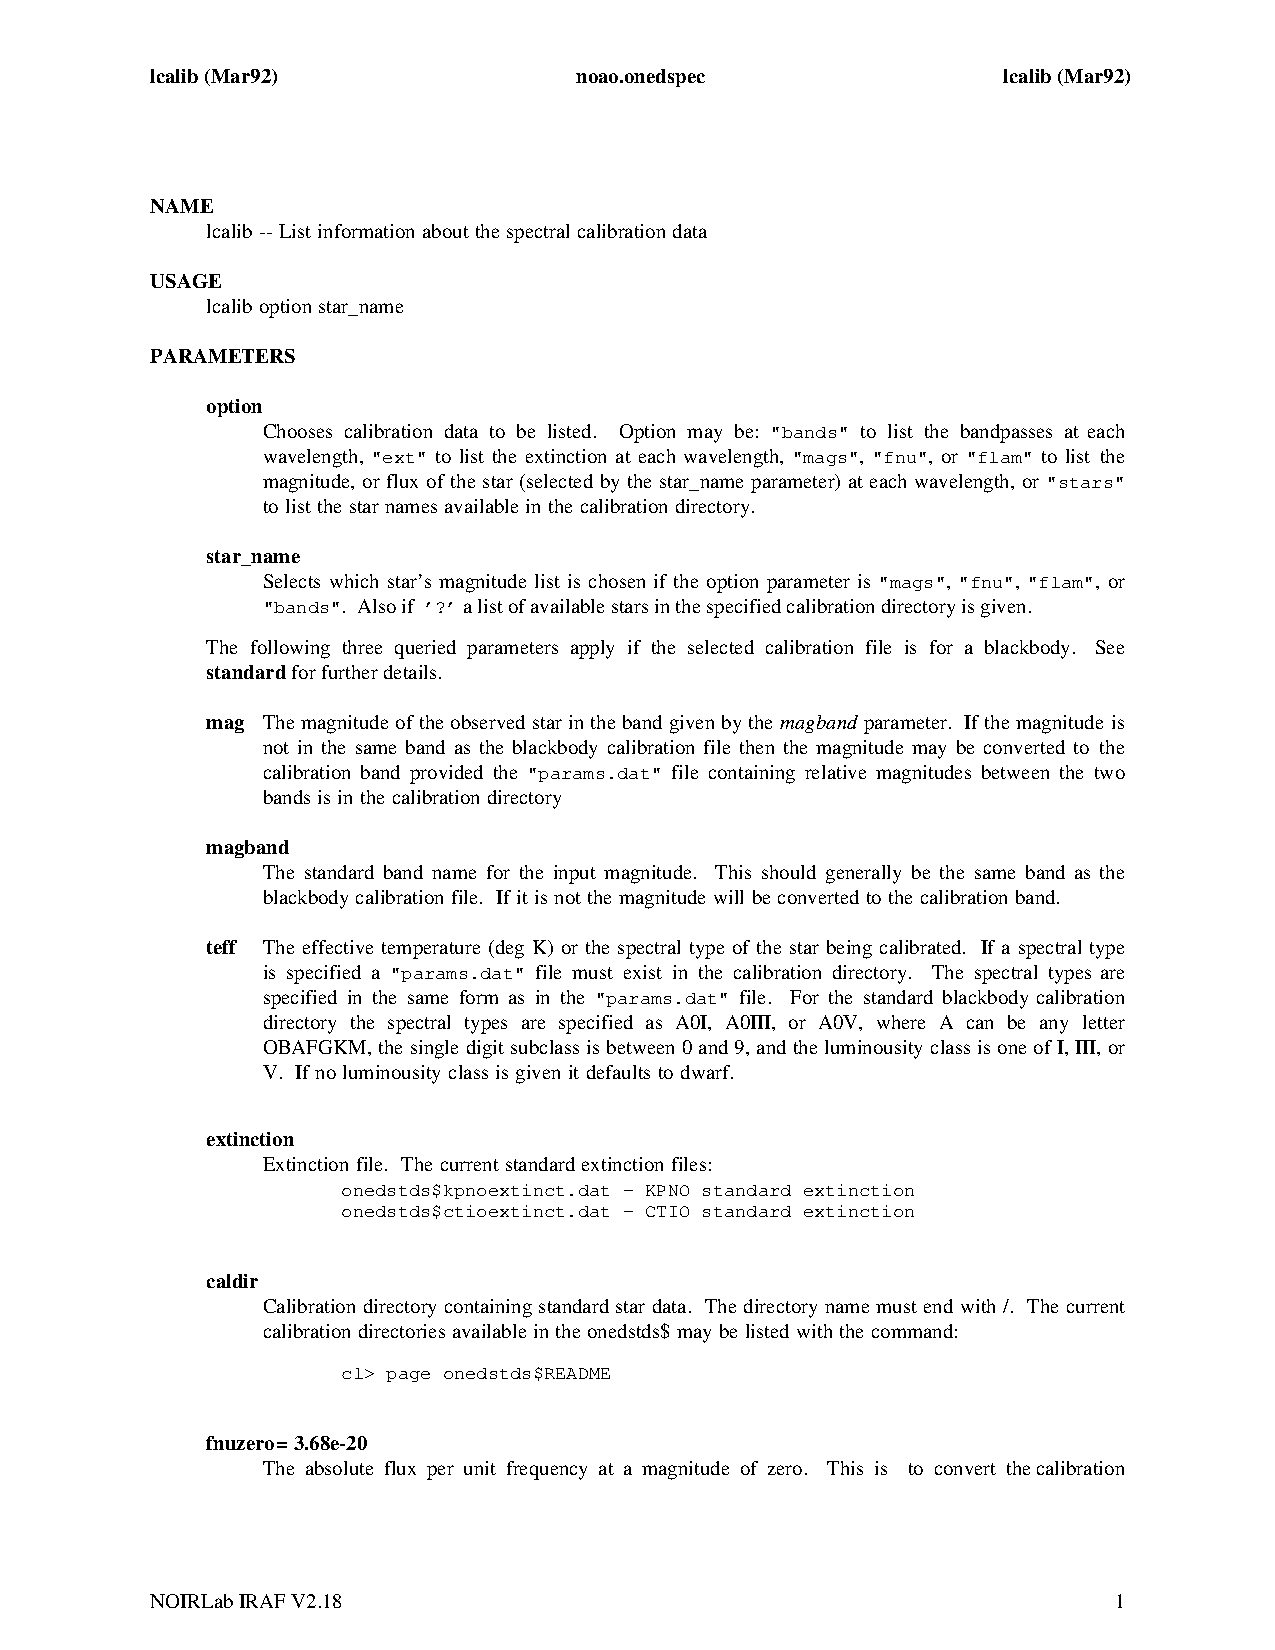
\includepdf[pages=-,addtotoc={1,section,1,lcalib,sec:lcalib}]{lcalib.pdf}

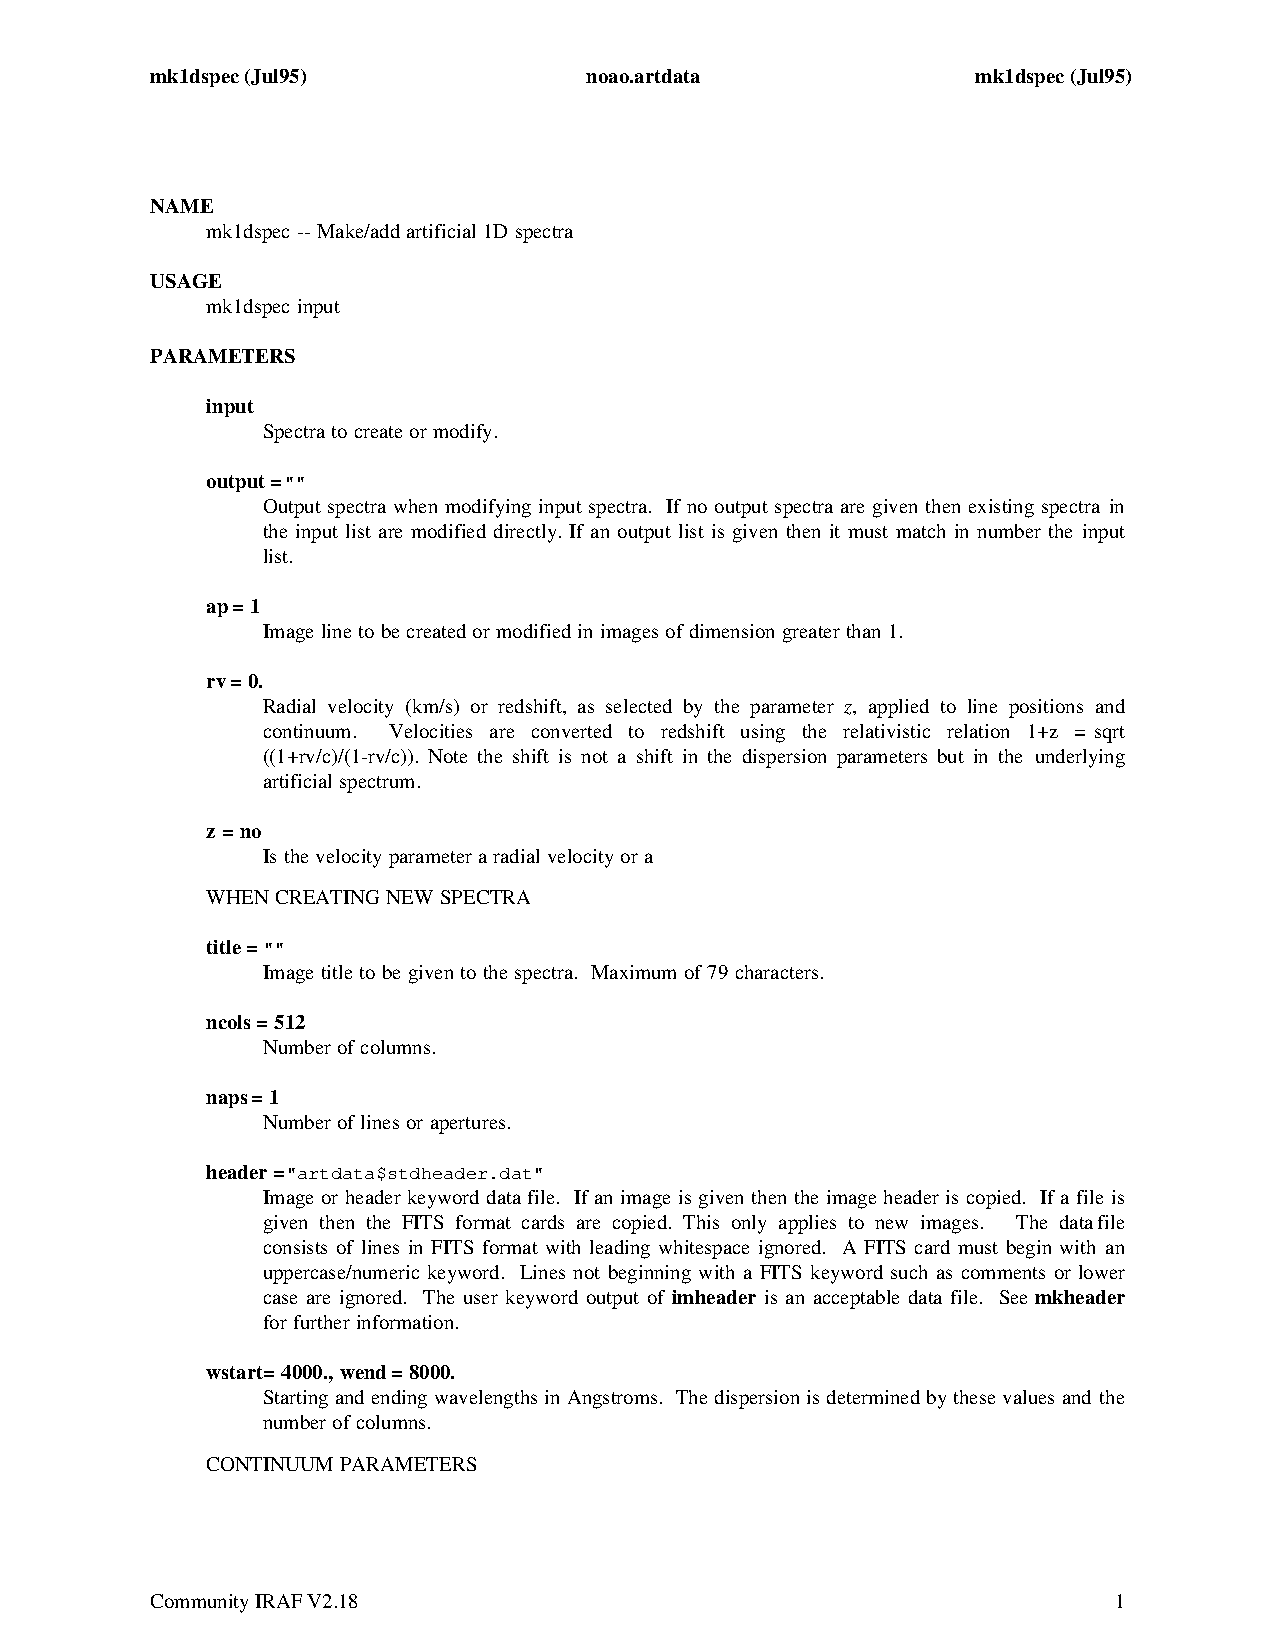
\includepdf[pages=-,addtotoc={1,section,1,mk1dspec,sec:mk1dspec}]{mk1dspec.pdf}

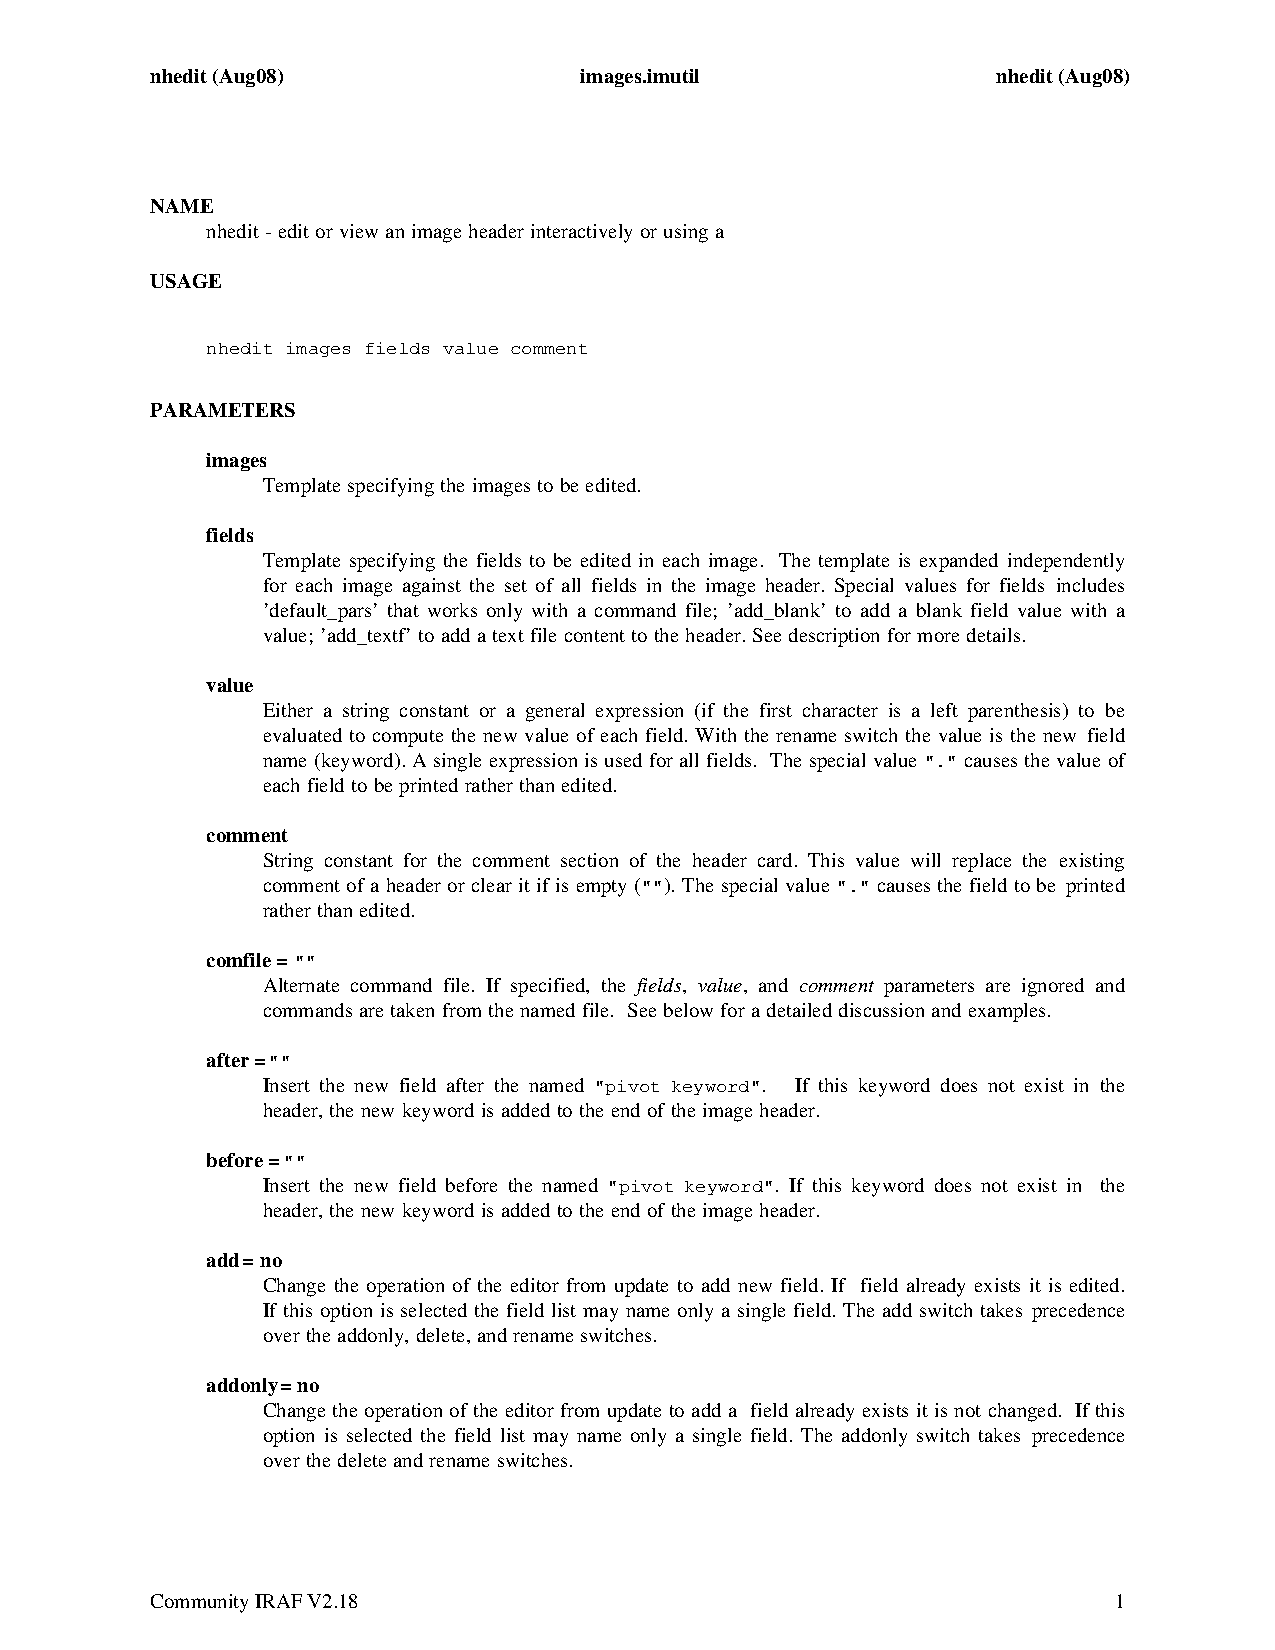
\includepdf[pages=-,addtotoc={1,section,1,nhedit,sec:nhedit}]{nhedit.pdf}

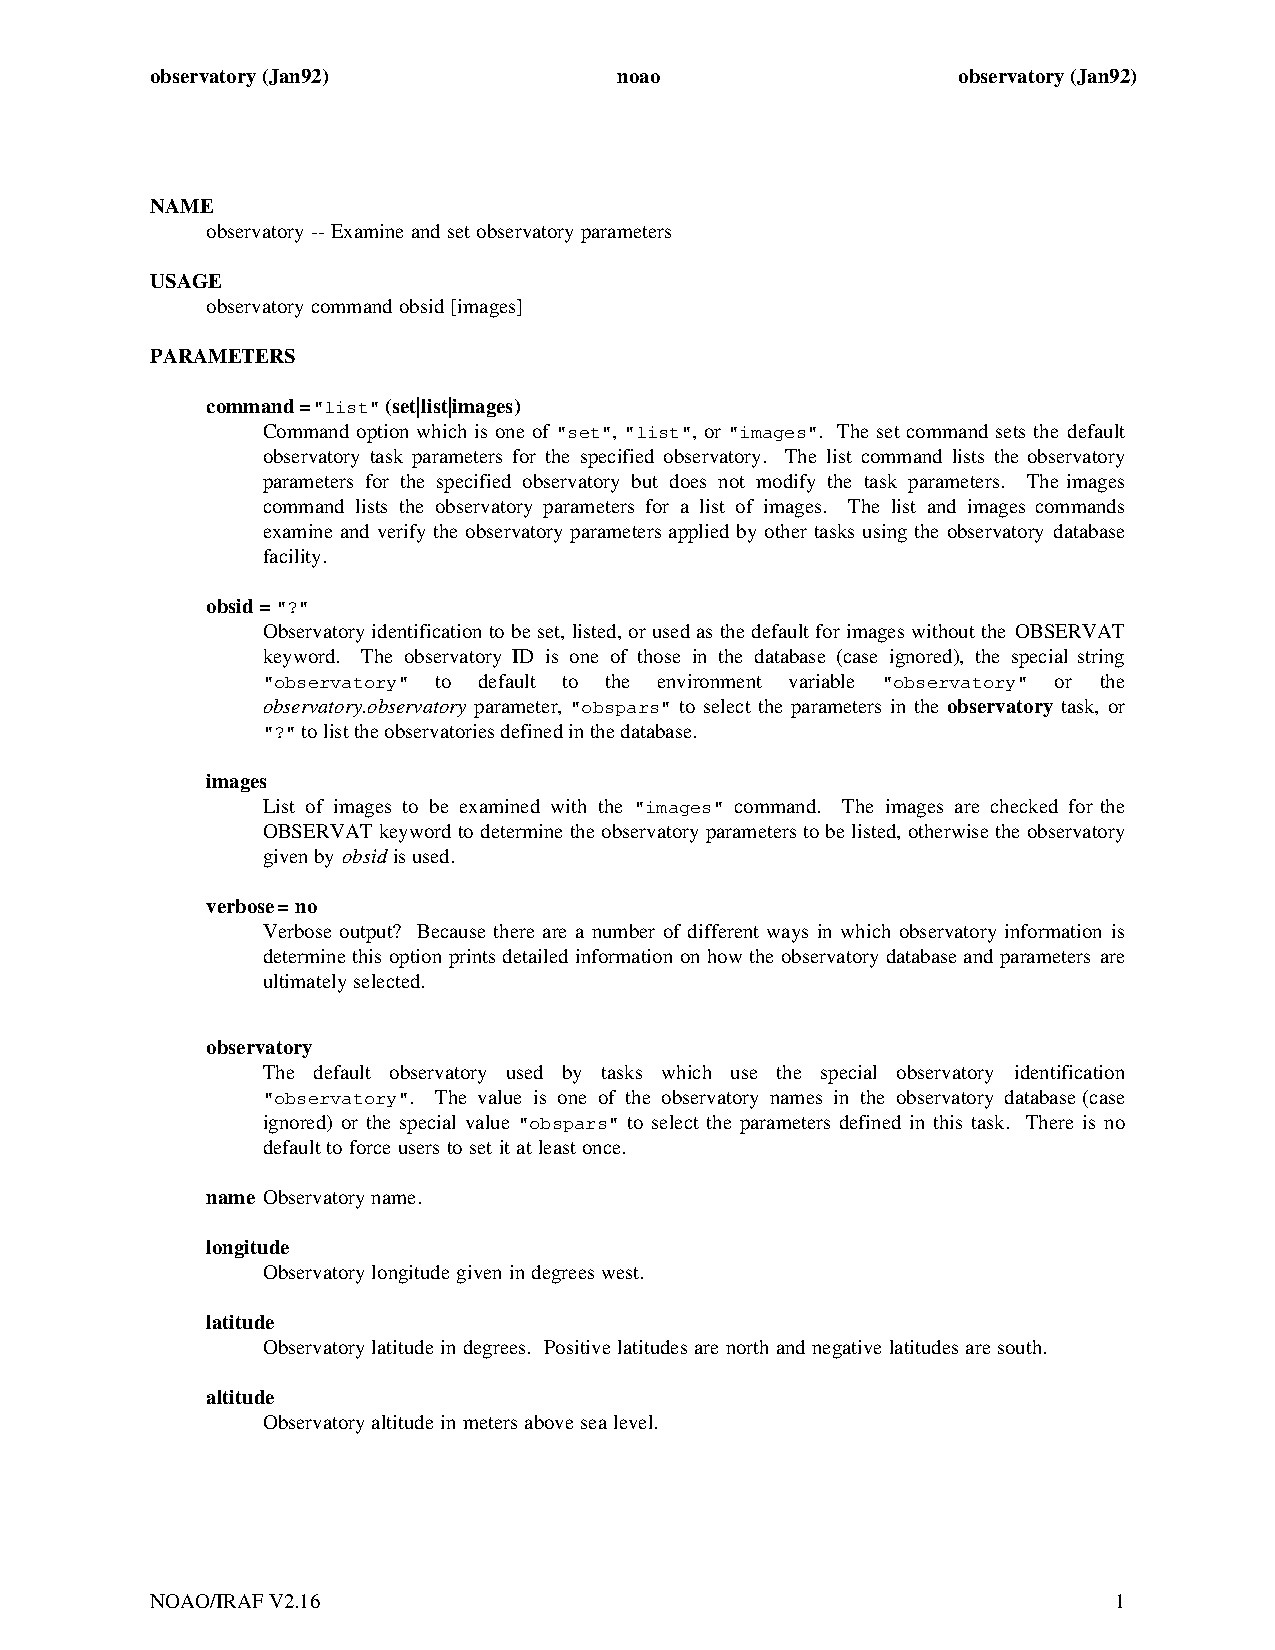
\includepdf[pages=-,addtotoc={1,section,1,observatory,sec:observatory}]{observatory.pdf}

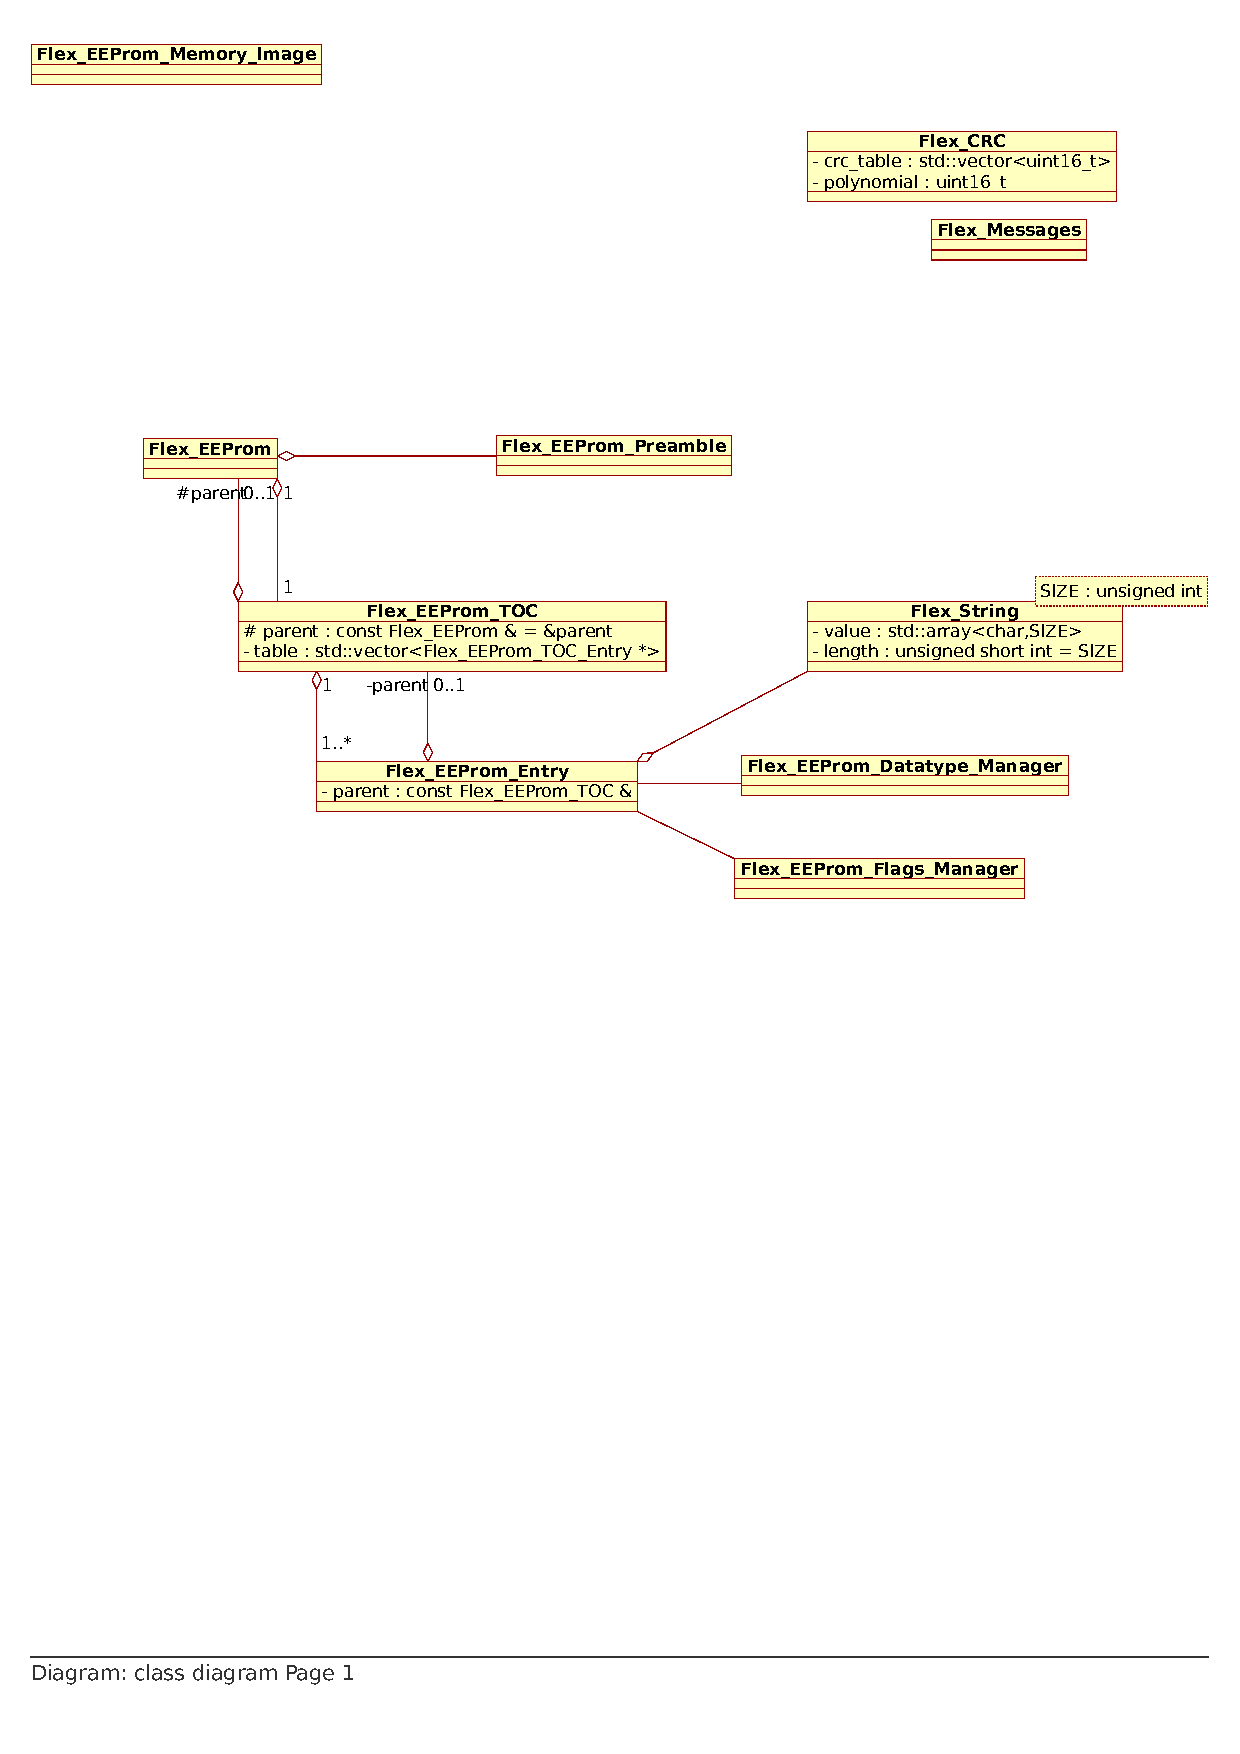
\includepdf[pages=-,addtotoc={1,section,1,print,sec:print}]{print.pdf}

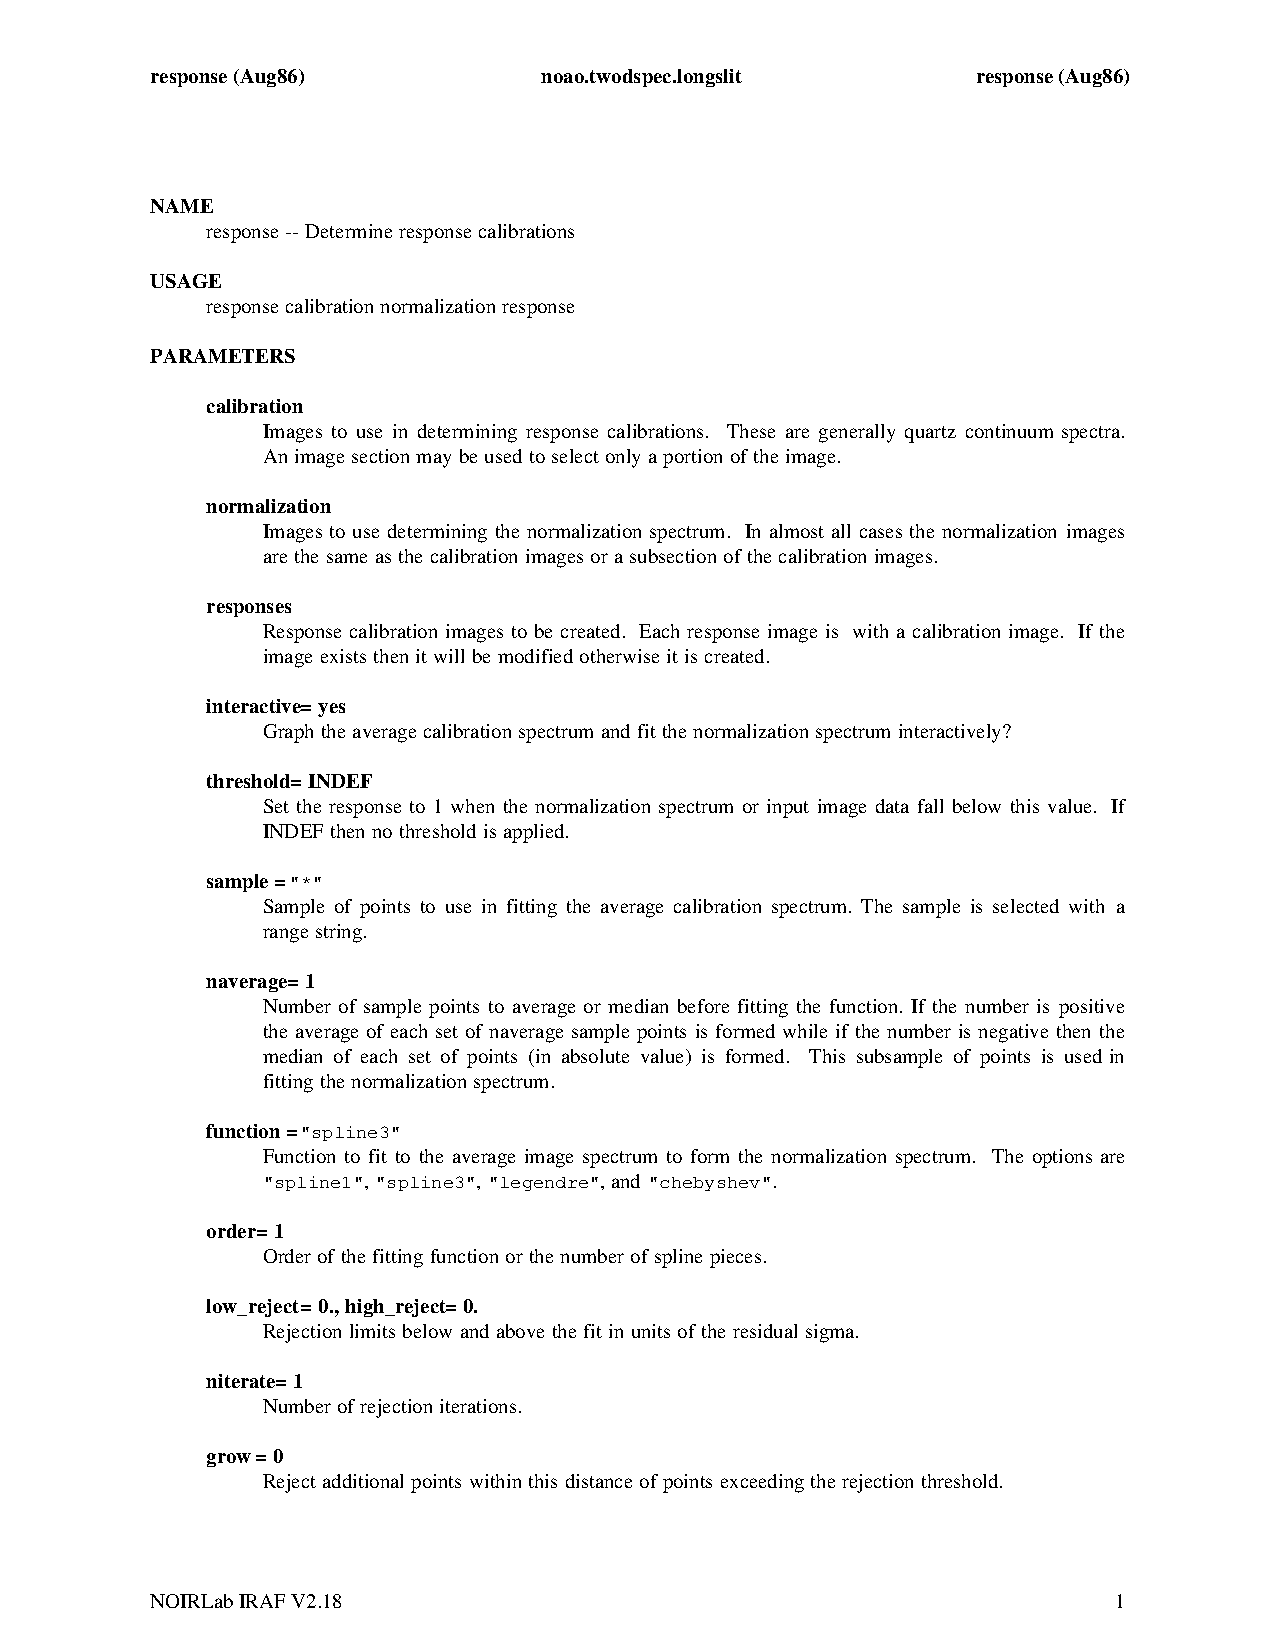
\includepdf[pages=-,addtotoc={1,section,1,response,sec:response}]{response.pdf}

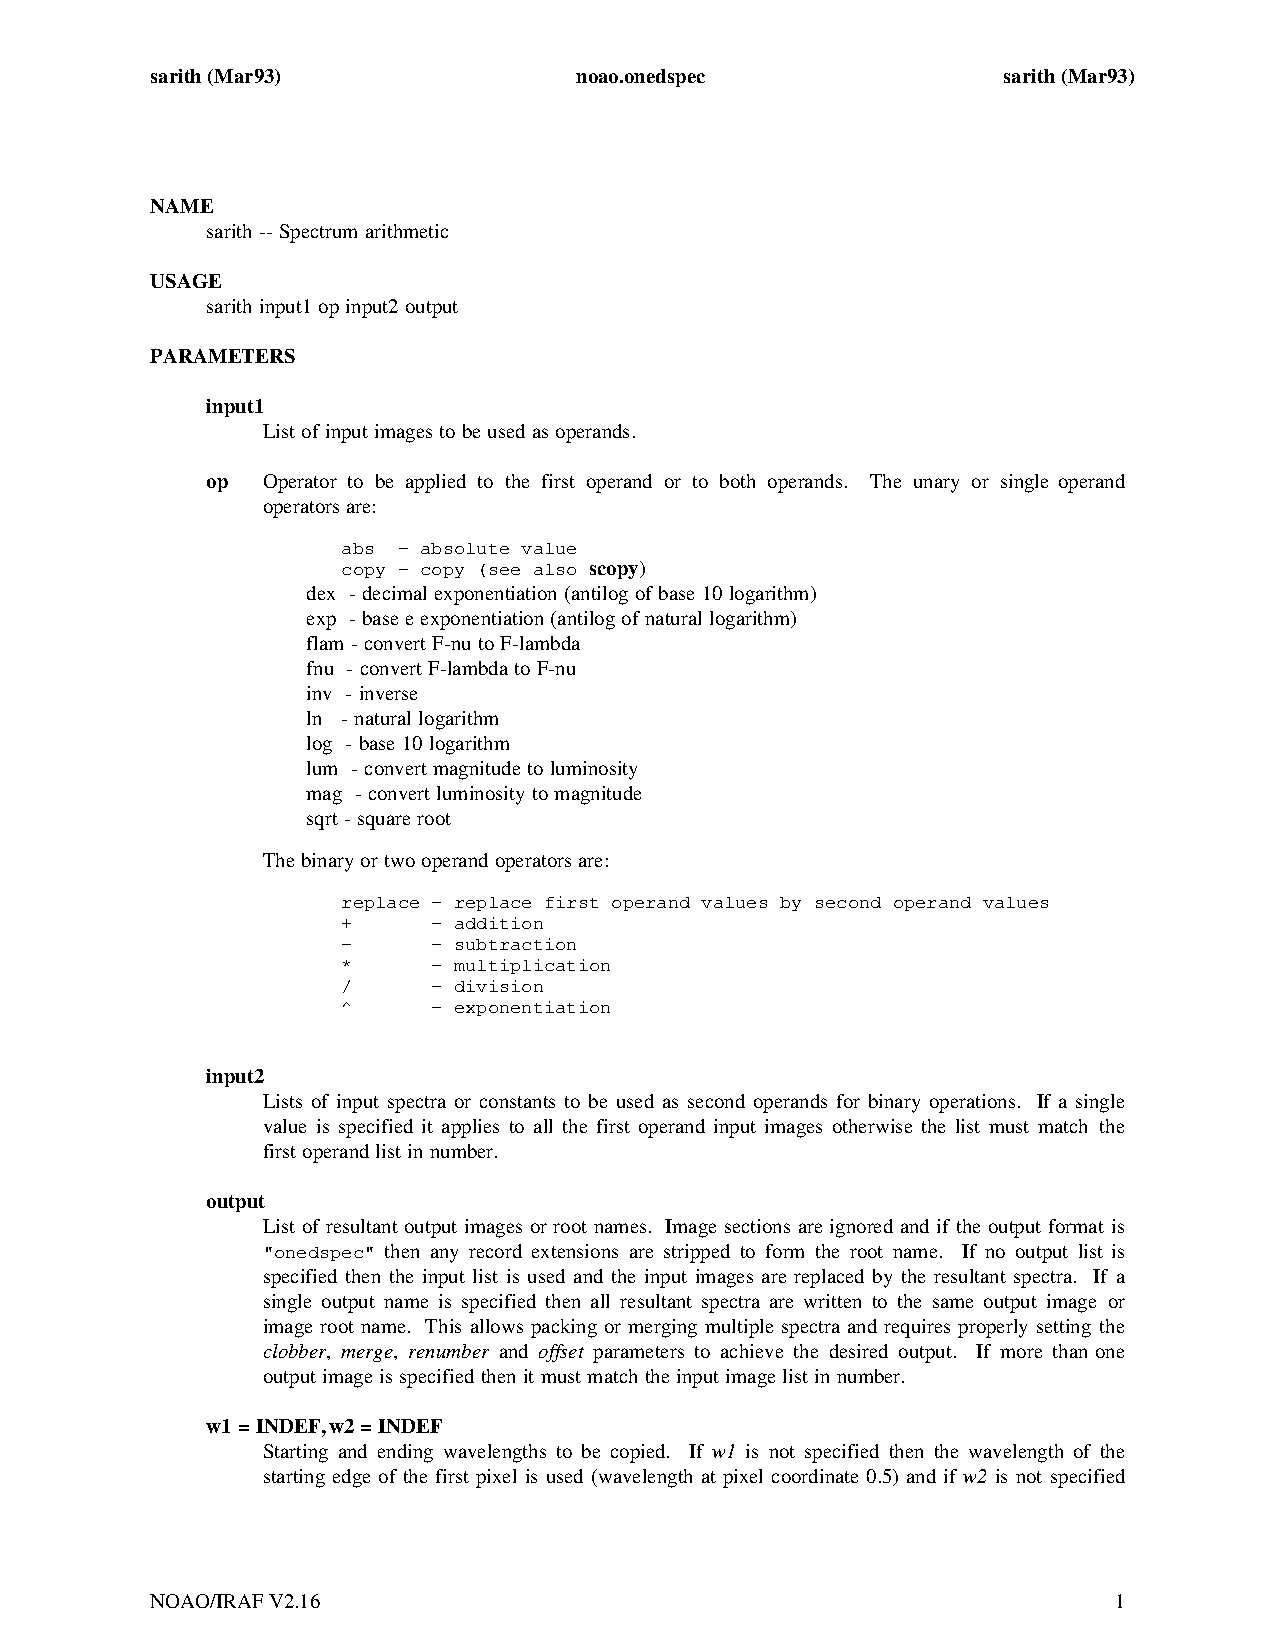
\includepdf[pages=-,addtotoc={1,section,1,sarith,sec:sarith}]{sarith.pdf}

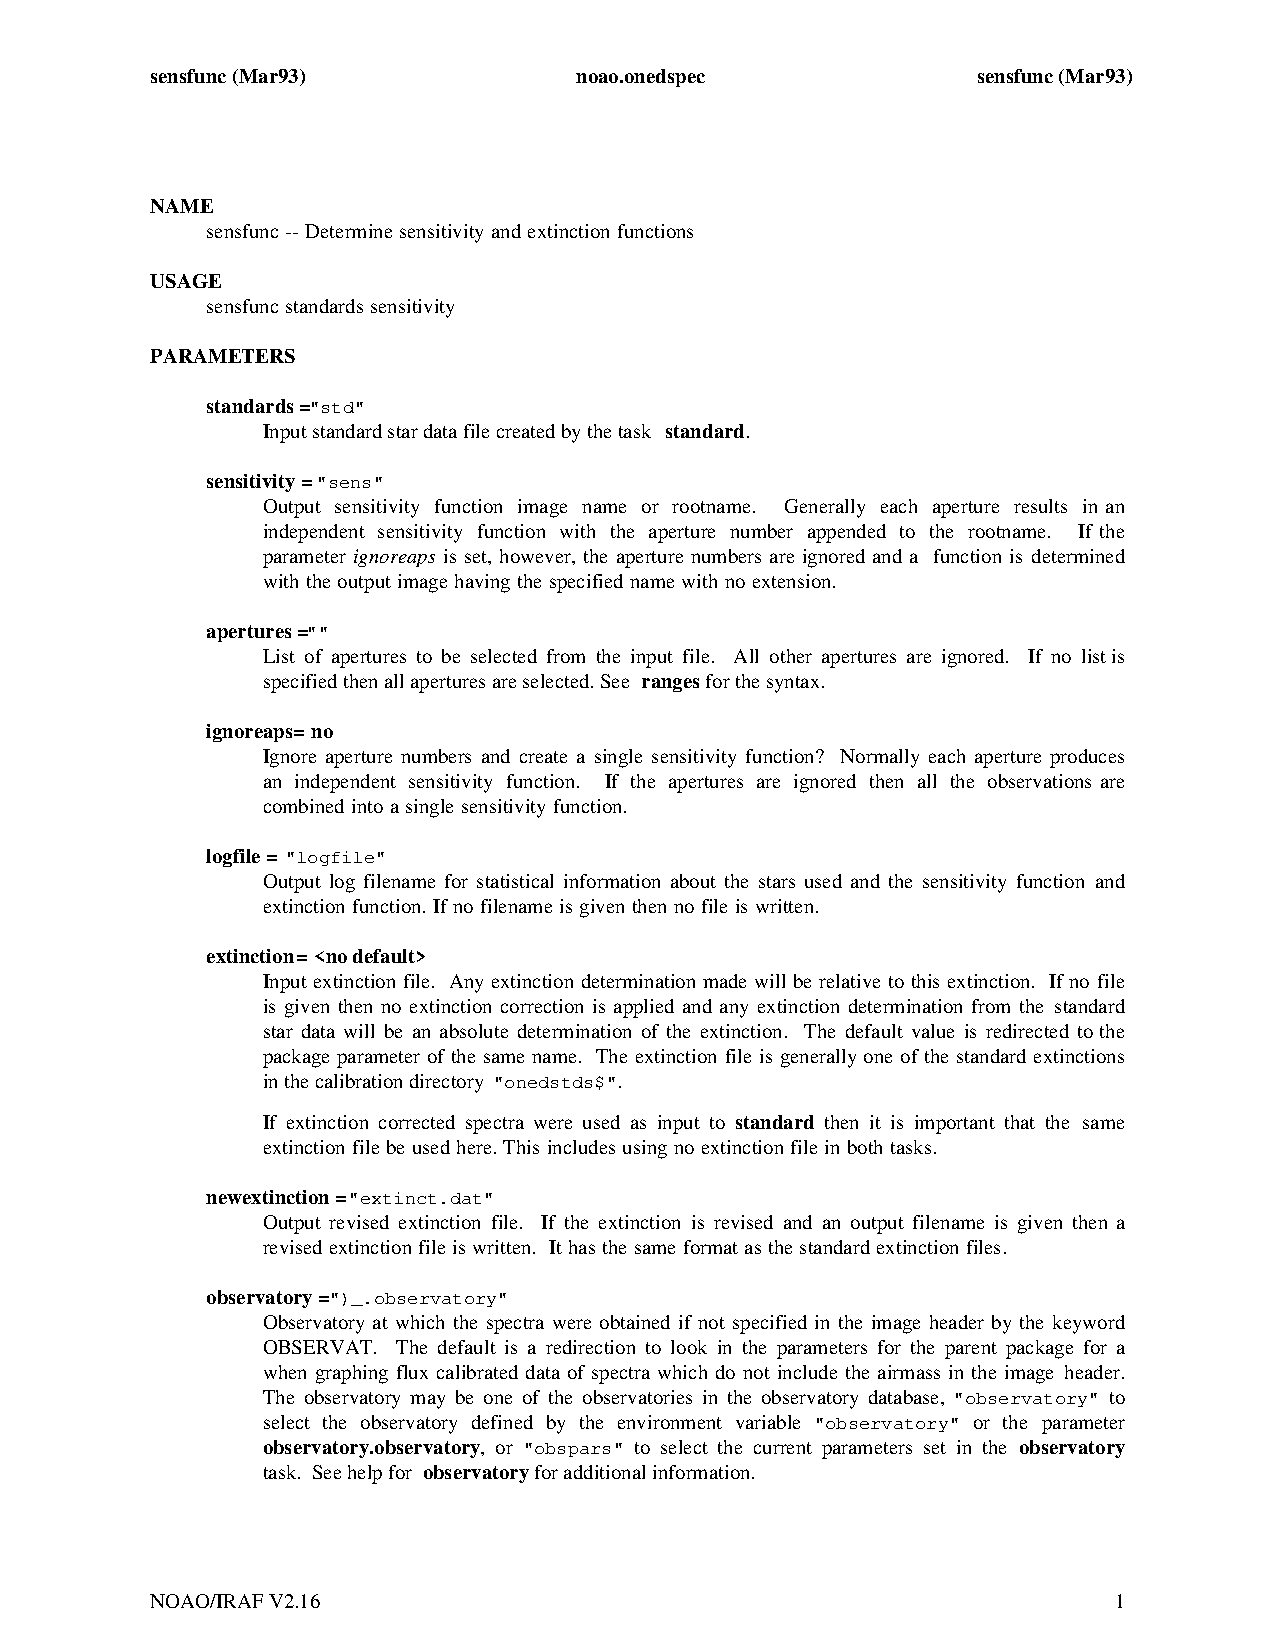
\includepdf[pages=-,addtotoc={1,section,1,sensfun,sec:sensfun}]{sensfun.pdf}

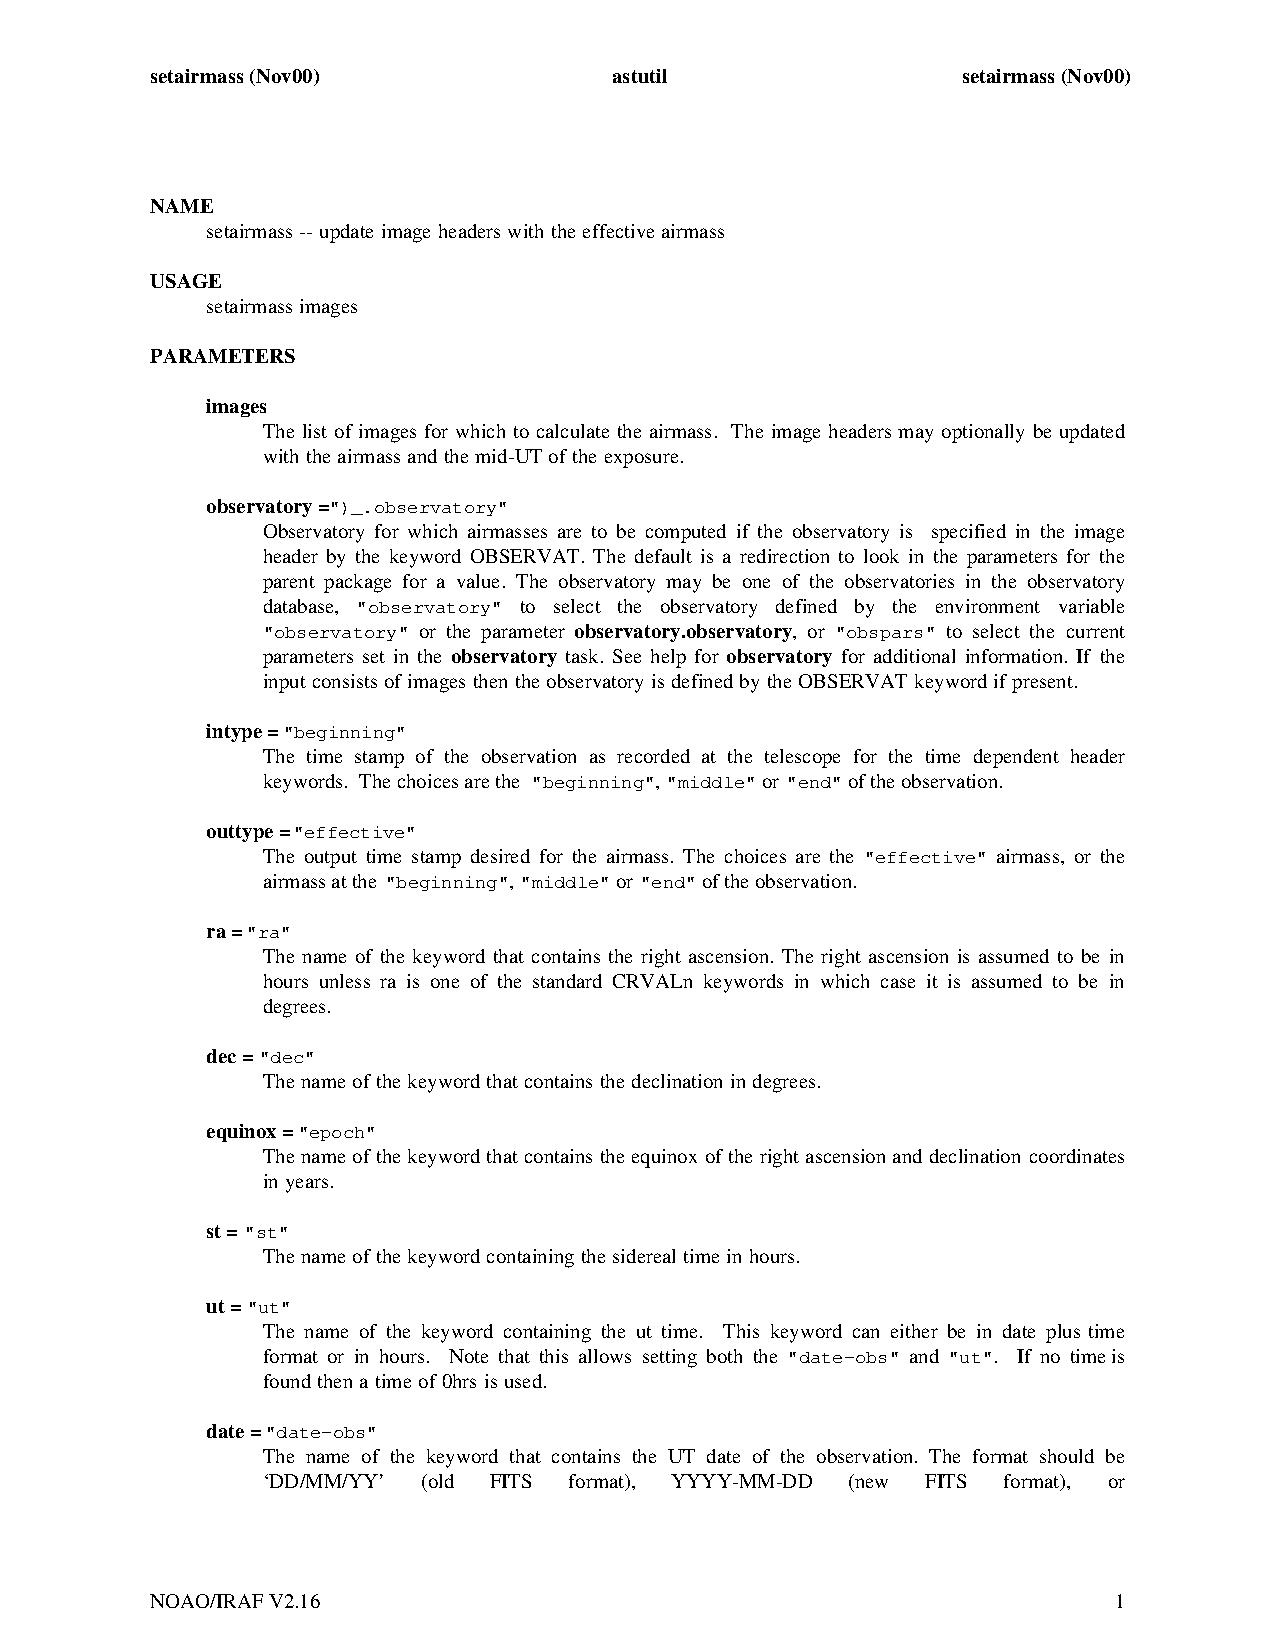
\includepdf[pages=-,addtotoc={1,section,1,setairmass,sec:setairmass}]{setairmass.pdf}

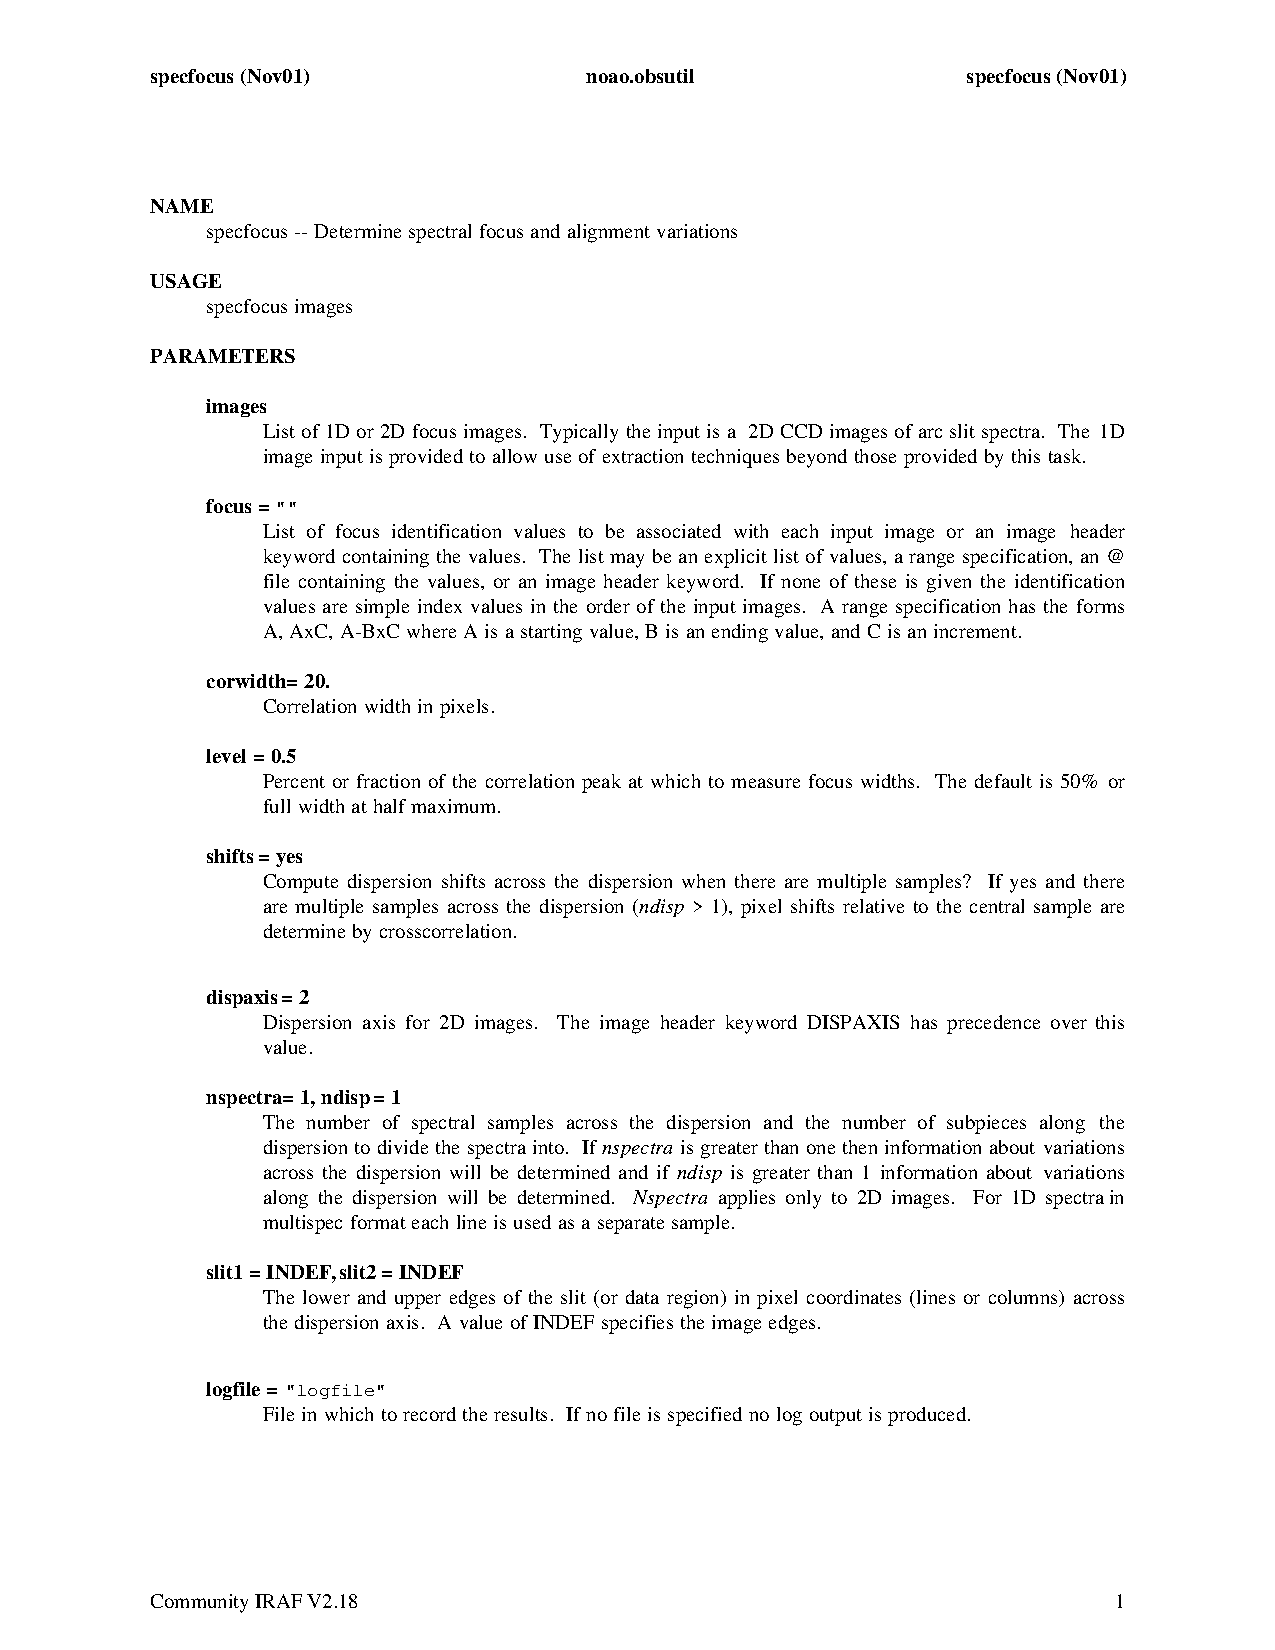
\includepdf[pages=-,addtotoc={1,section,1,specfocus,sec:specfocus}]{specfocus.pdf}

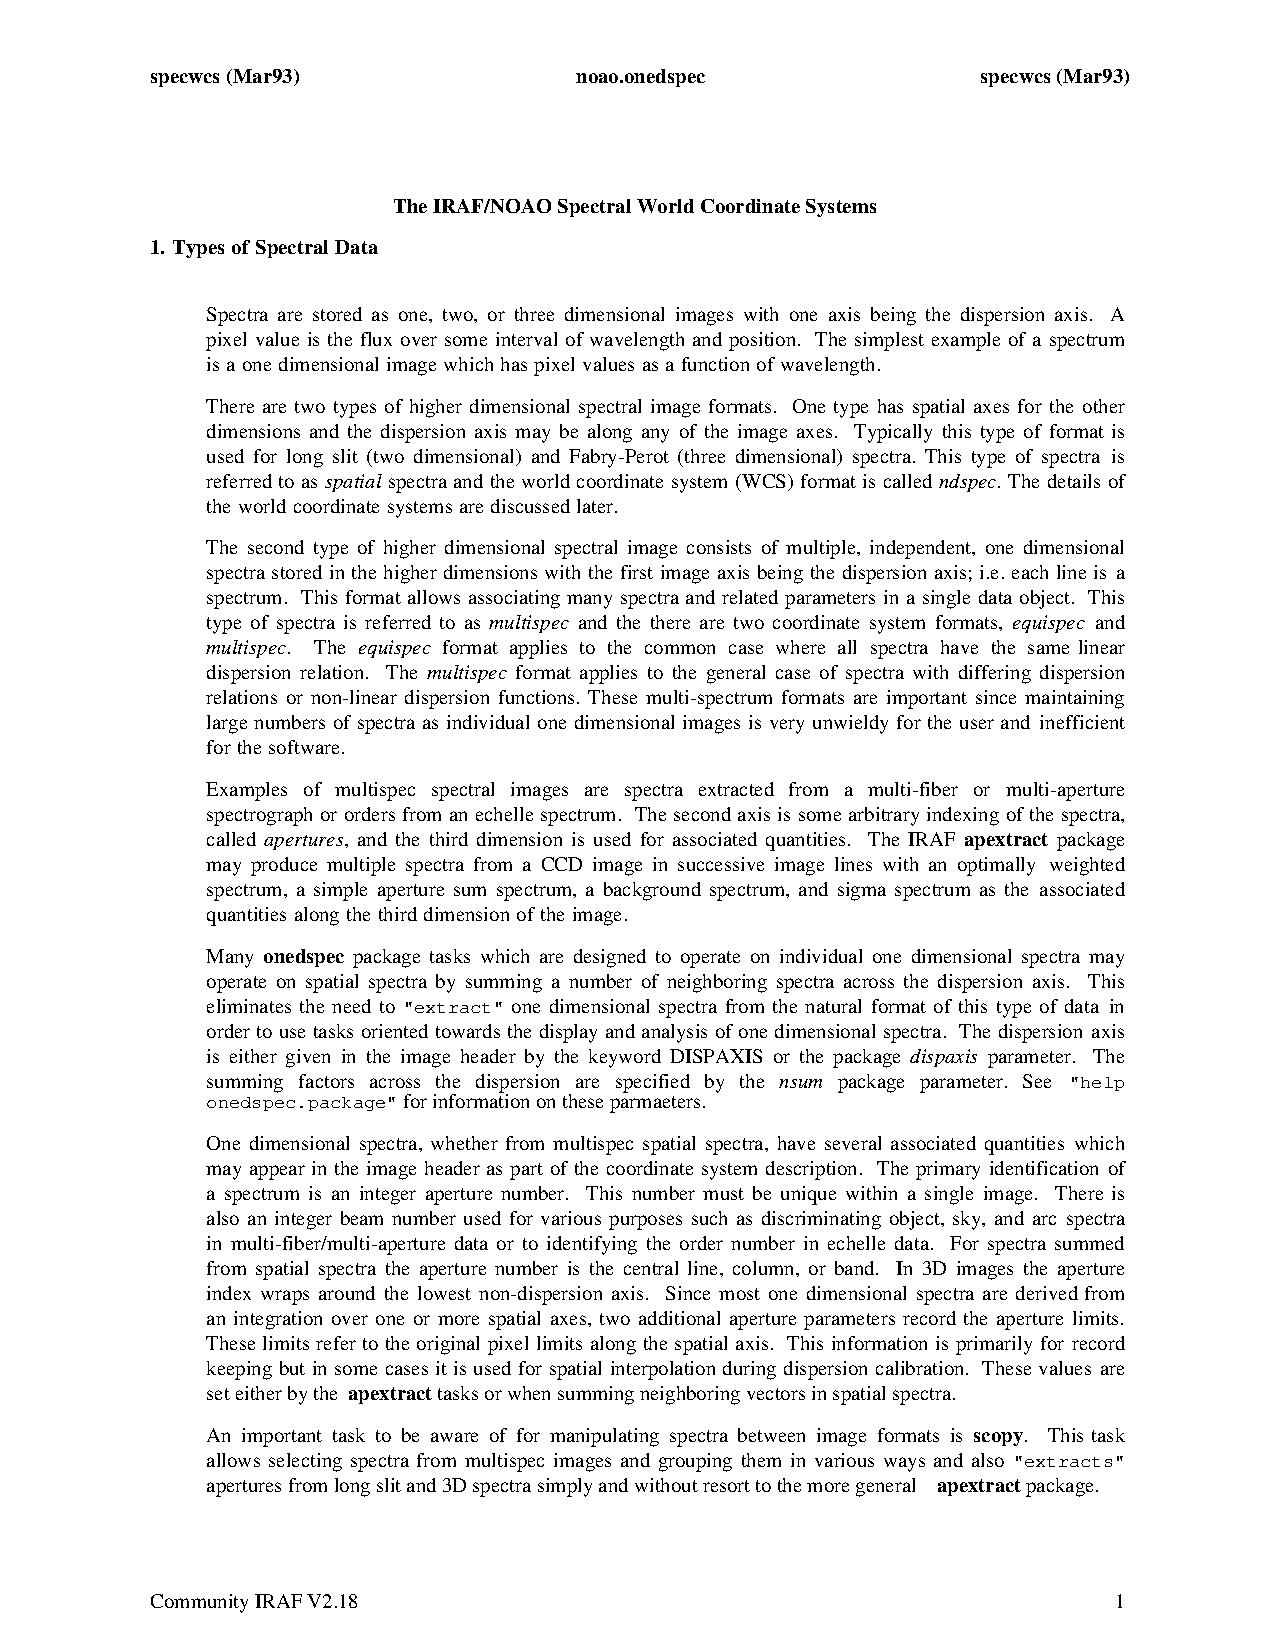
\includepdf[pages=-,addtotoc={1,section,1,specwcs,sec:specwcs}]{specwcs.pdf}

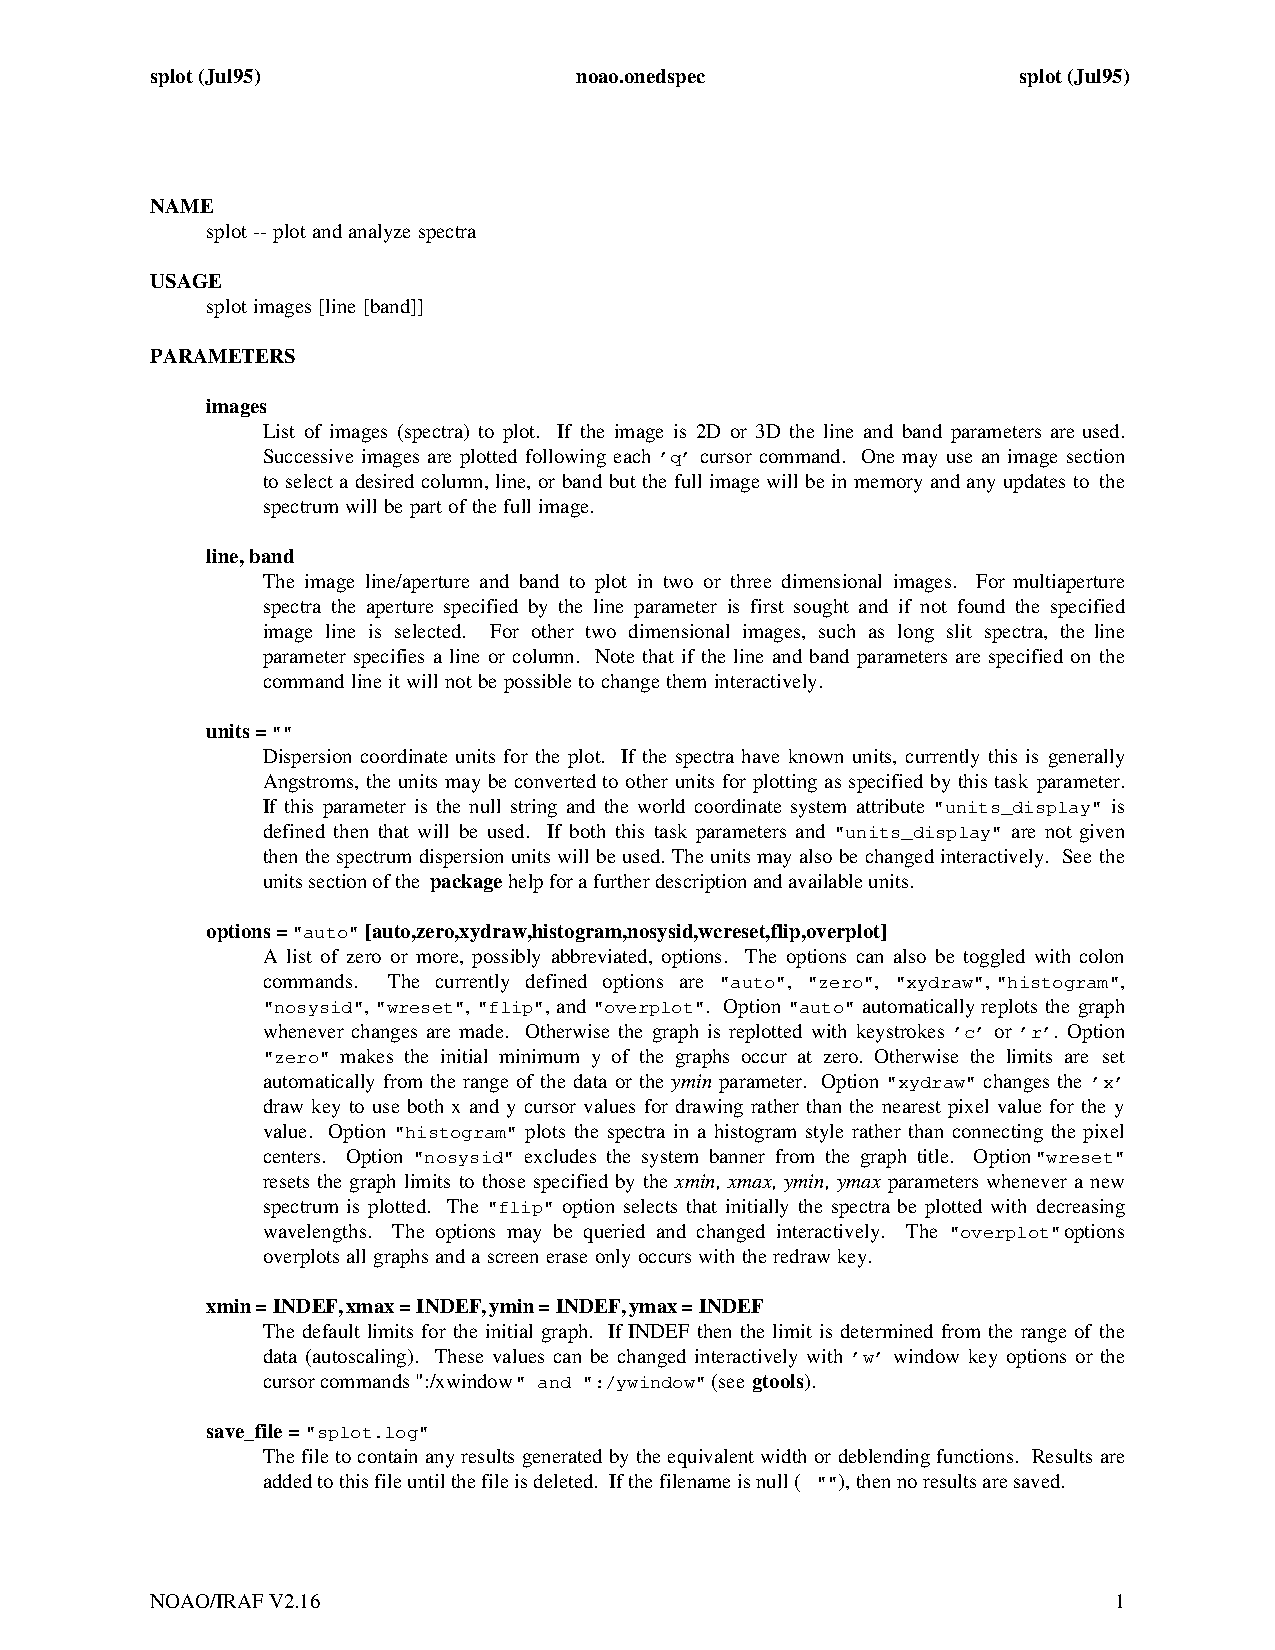
\includepdf[pages=-,addtotoc={1,section,1,splot,sec:splot}]{splot.pdf}

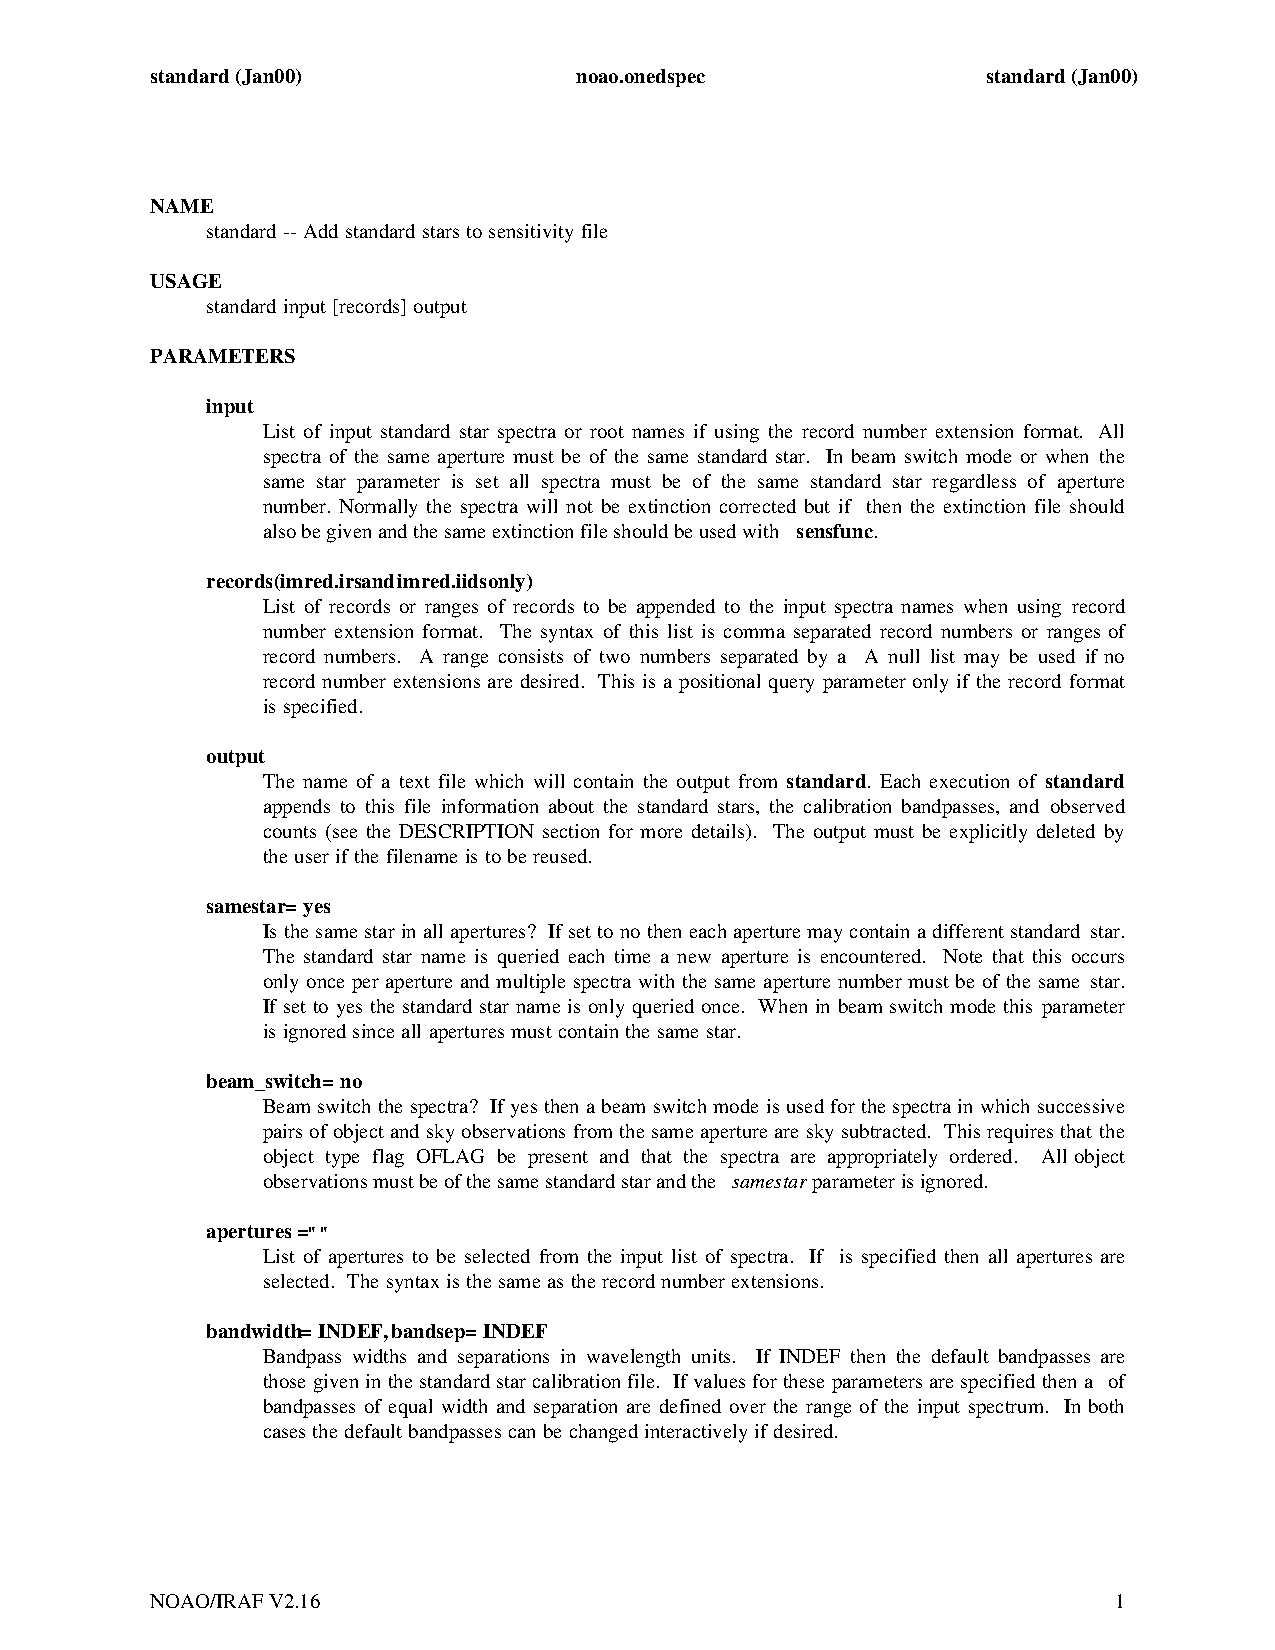
\includepdf[pages=-,addtotoc={1,section,1,standard,sec:standard}]{standard.pdf}

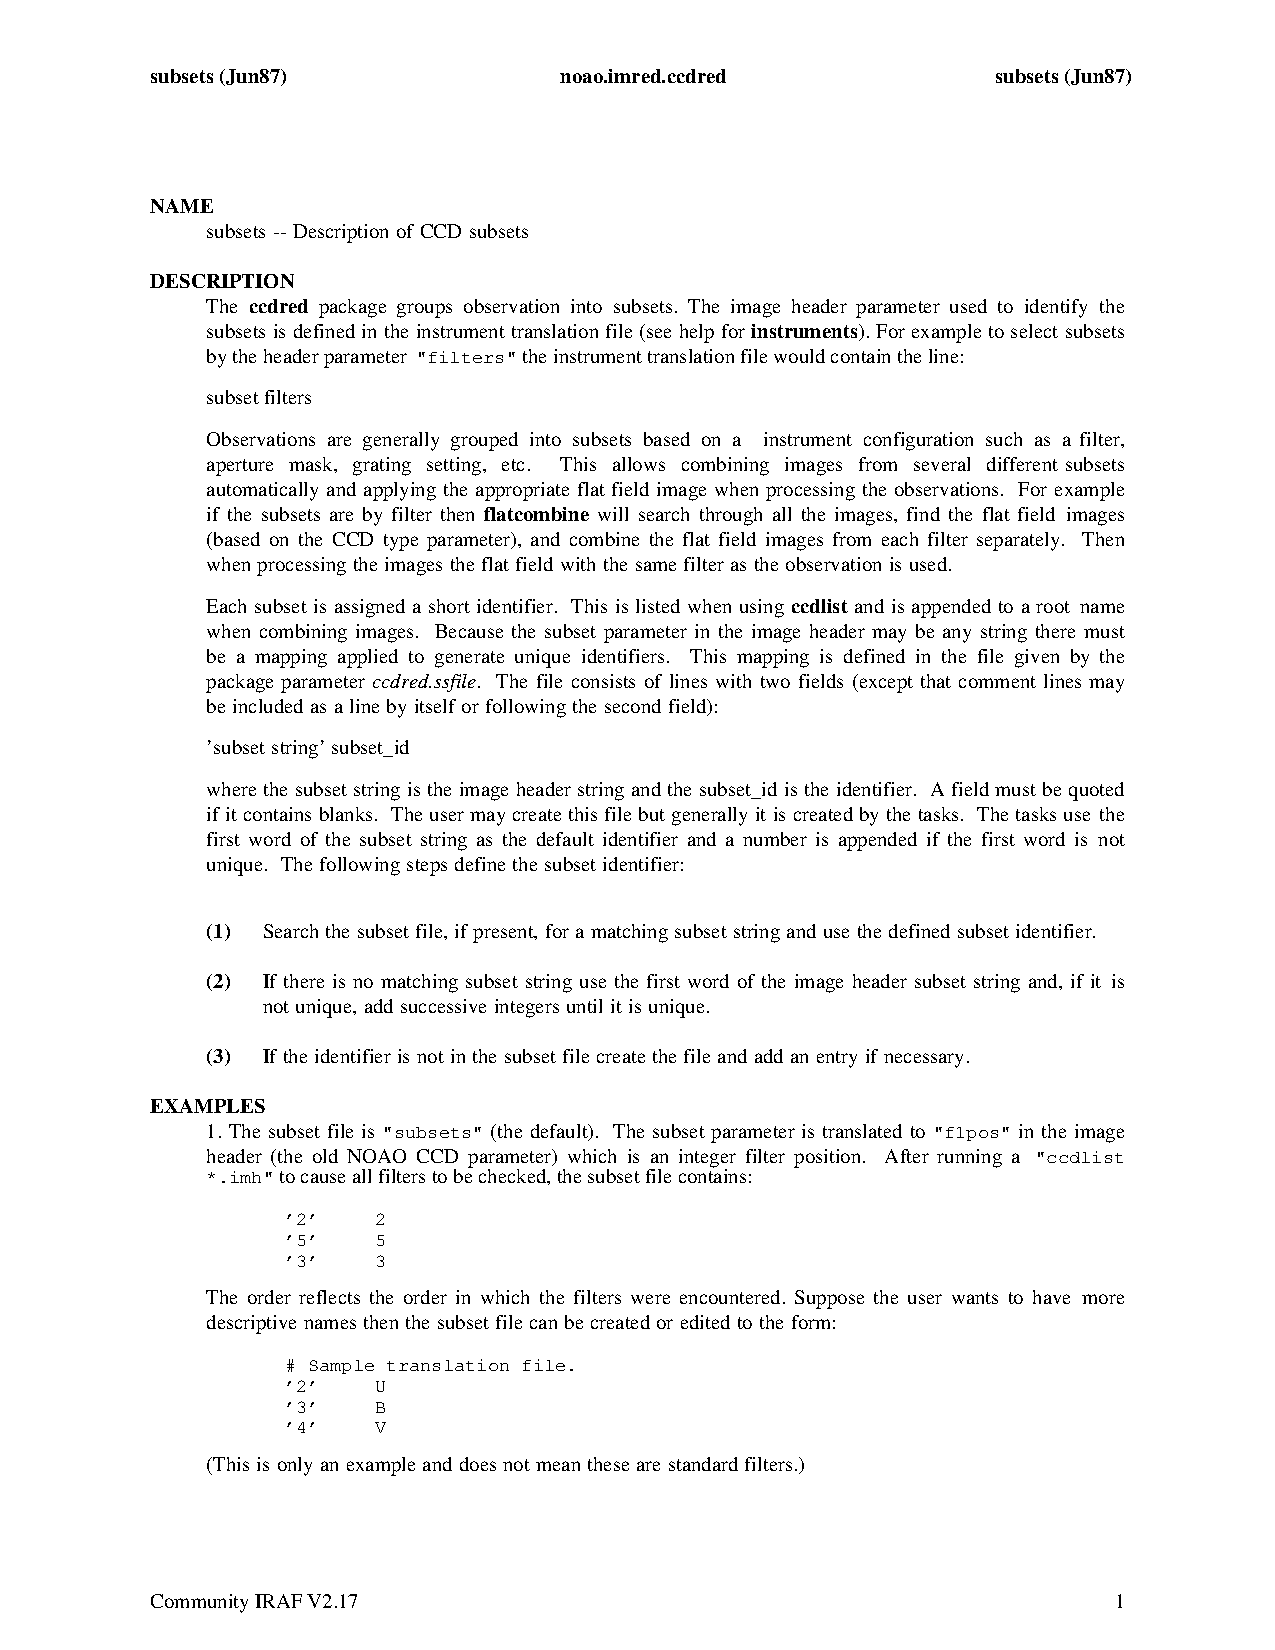
\includepdf[pages=-,addtotoc={1,section,1,subsets,sec:subsets}]{subsets.pdf}

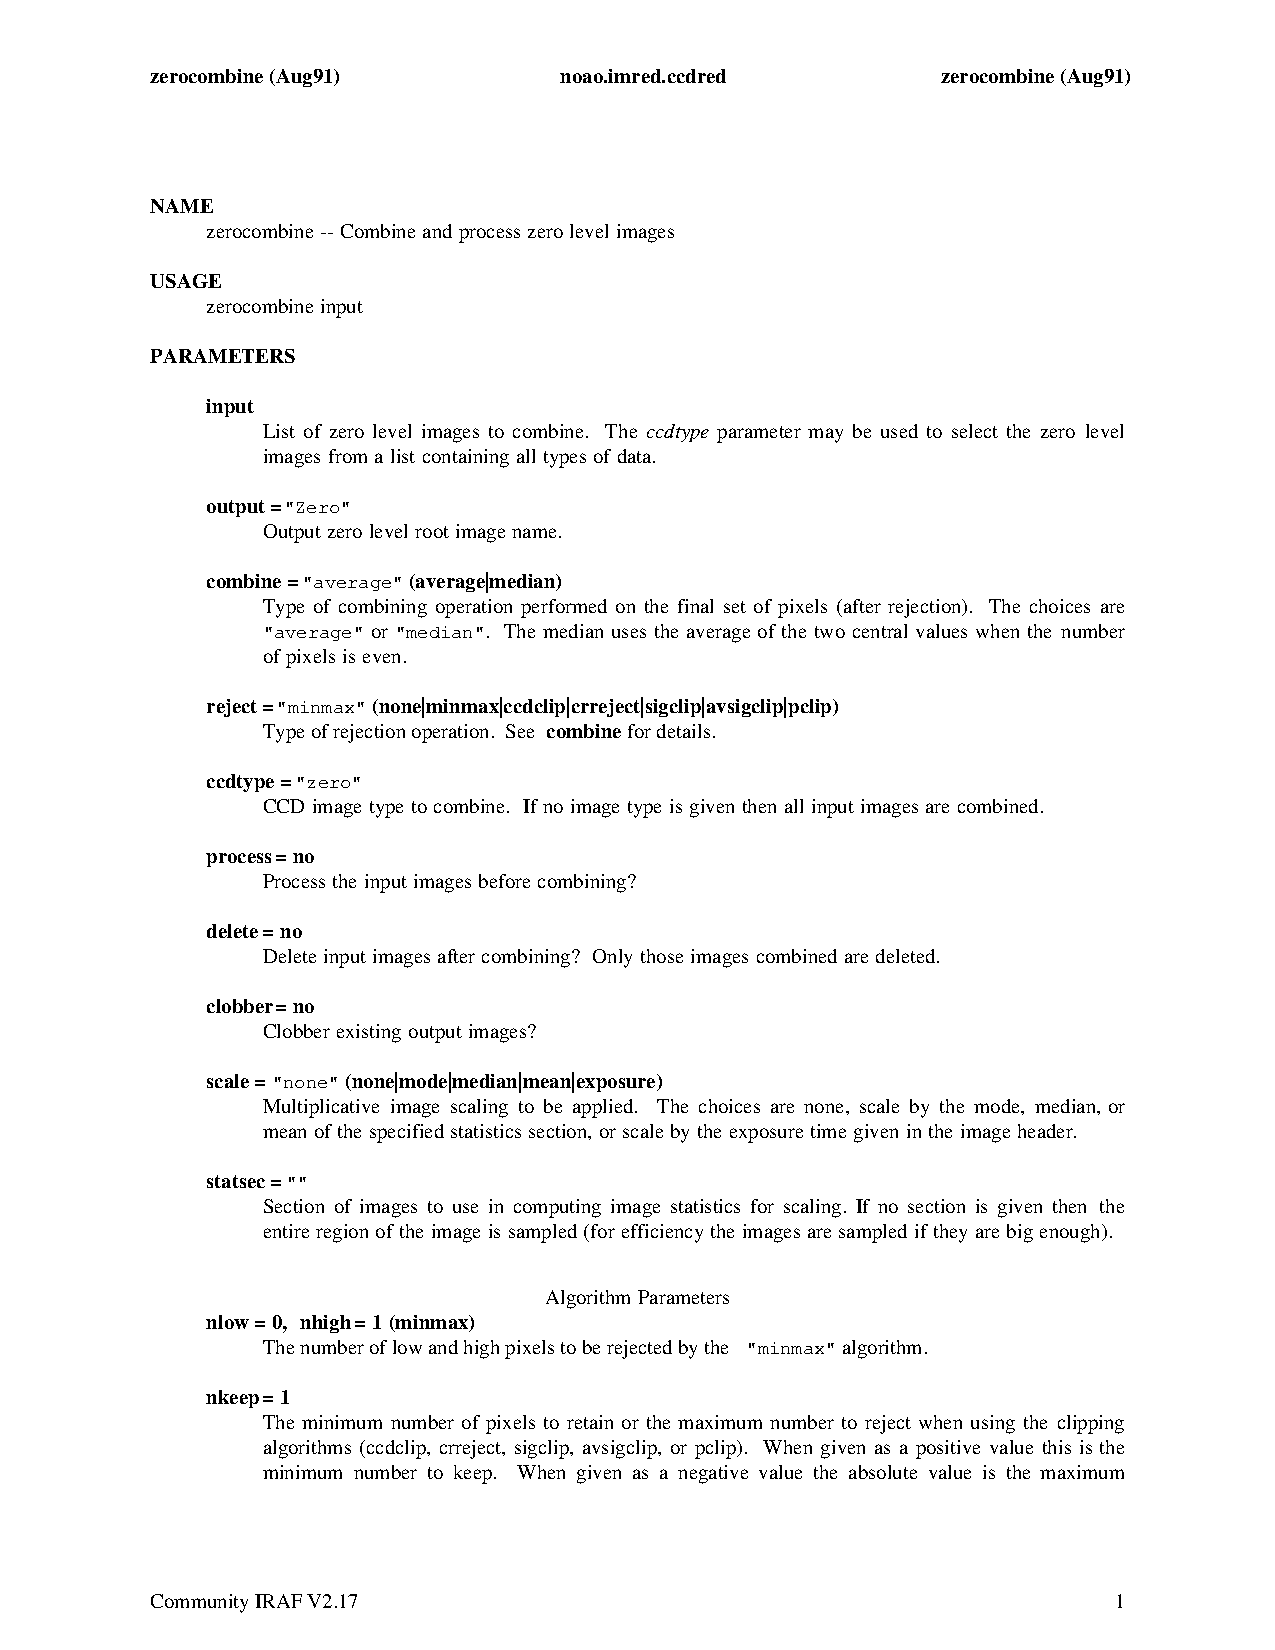
\includepdf[pages=-,addtotoc={1,section,1,zerocombine,sec:zerocombine}]{zerocombine.pdf}




%%\appendix
%%\renewcommand \thesection{\Alph{section}}

%% use a bibitem approach to the references publications etc.
%% (wg-bibitem)

%%\clearpage
%%\addcontentsline{toc}{section}{References}
%%\renewcommand*{\refname}{My Bibliography and References}
%%\bibliographystyle{apalike}	% bibliographystyle{apalike} and \usepackage{natbib}
%%\bibliography{MasterBib}	% expects file "MasterBib.bib"



%%\begin{thebibliography}{80}
%%\usepackage{natbib}   %% bibitems
%%\end{thebibliography}

%%\clearpage
%%\addcontentsline{toc}{section}{Index}
%%\printindex %% www.cs.usask.ca/resources/tutorials/latex/notes/toc-index.pdf

% /home/wayne/Desktop/Manuals/IRAF/man/BonMotsMan.tex

%% (wg-texdoc-endnotes)
\end{document}
